% !TEX TS-program = XeLaTeX
% Commands for running this example:
% 	 xelatex main
% 	 bibtex   main
%    xindy -L persian-variant1 -C utf8 -M texindy main.idx
% 	 xelatex main
% 	 xelatex main
% End of Commands

%        نمونه پایان‌نامه آماده شده با استفاده از کلاس HSU-Thesis، برای پایان‌نامه‌های دانشگاه حکیم سبزواری
% 		محمود امین‌طوسی، دانشگاه حکیم سبزواری، http://mamintoosi.ir
% 		گروه پارسی‌لاتک  http://www.parsilatex.com

%----------------------------------------------------------------------------------------------
\RequirePackage[final]{graphicx}
%        اگر مایلید پایان‌نامه شما دورو باشد به جای oneside  در خط زیر از twoside استفاده کنید
%        اگر قصد نوشتن پروژه کارشناسی را دارید، در خط زیر به جای msc، کلمه bsc و اگر قصد نوشتن پروژه دکترا
%        را دارید، کلمه phd را قرار دهید. کلیه تنظیمات لازم، به طور خودکار، اعمال می‌شود.
% 		و اگر مایلید نسخه پیش نویس را داشته باشید draft را به گزینه ها اضافه کنید.
\documentclass[oneside,openany,dvipsnames,msc,12pt]{HSU-Thesis} %,draft

% مشخصات پایان‌نامه را در فایلهای faTitle و enTitle وارد نمایید.

%       فایل commands.tex را مطالعه کنید؛ چون دستورات مربوط به فراخوانی بسته زی‌پرشین 
%       و دیگر بسته‌ها و ... در این فایل قرار دارد و بهتر است که با نحوه استفاده از آنها آشنا شوید.
% !TEX TS-program = XeLaTeX
% !TeX root=main.tex
% در این فایل، دستورها و تنظیمات مورد نیاز، آورده شده است.
%-------------------------------------------------------------------------------------------------------------------

% در ورژن جدید زی‌پرشین برای تایپ متن های ریاضی، این سه بسته، حتماً باید فراخوانی شود
\usepackage{amsthm,amssymb,amsmath}
% بسته‌ای برای تنطیم حاشیه‌های بالا، پایین، چپ و راست صفحه
\usepackage[top=30mm, bottom=30mm, left=25mm, right=35mm]{geometry}
% بسته  ای برای ظاهر شدن شکل ها و تصاویر متن
\usepackage{graphicx}
\usepackage{pdfpages}
% بسته‌ای برای رسم کادر
%\usepackage{framed} 
% بسته  ای برای چاپ شدن خودکار تعداد صفحات در صفحه «معرفی پایان‌نامه»
%\usepackage{lastpage}
% hyperref: بسته  و دستوراتی برای ایجاد لینک های رنگی با امکان جهش
% بررسی حالت پیش نویس
\usepackage{ifdraft}
\ifdraft
{%
    \usepackage[pagebackref=true,colorlinks,linkcolor=blue,citecolor=blue,final]{hyperref}
    \usepackage[firstpage]{draftwatermark}
\SetWatermarkText{\ \ \ پیش‌نویس}
\SetWatermarkScale{1.2}
}
{
 % اگر مایلید در نسخه چاپی هم لینکها رنگی باشند، رنگهای دستور زیر را مطابق دستور شش خط بالاتر تنظیم نمایید.
   \usepackage[pagebackref=false,colorlinks,linkcolor=black,citecolor=black,urlcolor=black]{hyperref}
}

\usepackage[obeyDraft]{todonotes}
\setlength{\marginparwidth}{2cm}

% بسته  لازم برای تنظیم سربرگ ها
\usepackage{fancyhdr}
%
\usepackage{setspace}
\usepackage{algorithm}
\usepackage{algorithmic}
\usepackage{subfigure}
\usepackage[subfigure]{tocloft}



% بسته موردنیاز برای رسم نمودارهای زیبا
\usepackage{tikz}
\usetikzlibrary{arrows,automata, shapes,positioning,matrix,calc}
\usepackage[object=vectorian]{pgfornament}
% بسته‌ای برای ظاهر شدن «مراجع» و «نمایه» در فهرست مطالب
\usepackage[nottoc]{tocbibind}
% دستورات مربوط به‌ایجاد نمایه
\usepackage{makeidx}
\makeindex
% رنگهای موردنیاز در کدنویسی
\usepackage{xcolor}
% بسته مورد نیاز برای نوشتن کدهای برنامه نویسی در نوشتار 
\usepackage[final]{listings}

\usepackage{tabularx}
\usepackage{hhline}
\usepackage{pbox}
\usepackage{caption}
\usepackage{rotating}
%\usepackage[thinlines]{easytable}

\usepackage{zref-perpage}% جهت شماره گذاری از یک زیرنویسها در هر صفحه
\zmakeperpage{footnote} % جهت شماره گذاری از یک زیرنویسها در هر صفحه

%\usepackage{xspace}
%%%%%%%%%%%%%%%%%%%%%%%%%%
% فراخوانی بسته زی‌پرشین و تعریف قلم فارسی و انگلیسی
\usepackage[extrafootnotefeatures,fontsize={13,16}]{xepersian}
\settextfont[BoldFont={IRLotusICEE_Bold.ttf}, BoldItalicFont={IRLotusICEE_BoldIranic.ttf}, ItalicFont={IRLotusICEE_Iranic.ttf},Scale=1.2]{IRLotusICEE.ttf}%{IRZar.ttf}

\setlatintextfont[Scale=1]{Times New Roman}

%%%%%%%%%%%%%%%%%%%%%%%%%%
%حل مشکل قلم ریاضی در تک‌لایو ۲۰۲۰ و ۲۰۲۱
\ExplSyntaxOn
\cs_set_eq:NN
\etex_iffontchar:D
\tex_iffontchar:D
\cs_undefine:N \c_one
\int_const:Nn \c_one { 1 }
\ExplSyntaxOff

\setmathdigitfont[Scale=1.2]{IRLotusICEE.ttf}
%%%%%%%%%%%%%%%%%%%%%%%%%%
% تعریف قلم های فارسی و انگلیسی اضافی برای استفاده در بعضی از قسمت‌های متن
\defpersianfont\titlefont[Scale=1]{IRTitr.ttf}
\setiranicfont[Scale=1.3]{IRLotusICEE_Iranic.ttf}				% ایرانیک، خوابیده به چپ
% \defpersianfont\nastaliq[Contextuals=Swash,Scale=1.2]{IranNastaliq}
%\setmathsfdigitfont{IRTitr.ttf}


% راستچین شدن todonotes
\presetkeys{todonotes}{align=right,textdirection=righttoleft}{}
\makeatletter
\providecommand\@dotsep{5}
\def\listtodoname{فهرست کارهای باقیمانده}
\def\listoftodos{\newpage\noindent{\Large\vspace{10mm}\textbf{\listtodoname}}\@starttoc{tdo}}
\renewcommand{\@todonotes@MissingFigureText}{شکل}
\renewcommand{\@todonotes@MissingFigureUp}{شکل}
\renewcommand{\@todonotes@MissingFigureDown}{جاافتاده}
\makeatother


\paragraphfootnotes   % برای افقی بودن زیرنویسها
%%%%%%%%%%%%%%%%%%%%%%%%%%
% دستوری برای حذف کلمه «چکیده»
\renewcommand{\abstractname}{}
% دستوری برای حذف کلمه «abstract»
%\renewcommand{\latinabstract}{}
% دستوری برای تغییر نام کلمه «اثبات» به «برهان»
\renewcommand\proofname{\textbf{برهان}}
% دستوری برای تغییر نام کلمه «کتاب نامه» به «فهرست منابع»
\renewcommand{\bibname}{فهرست منابع}
% دستوری برای تعریف واژه‌نامه انگلیسی به فارسی
\newcommand\persiangloss[2]{#1\dotfill\lr{#2}\\}
% دستوری برای تعریف واژه‌نامه فارسی به انگلیسی 
\newcommand\englishgloss[2]{#2\dotfill\lr{#1}\\}
% تعریف دستور جدید «\پ» برای خلاصه نویسی جهت نوشتن عبارت «پروژه/پایان‌نامه/رساله»
\newcommand{\پ}{پروژه/ پایان‌نامه/ رساله }

%\newcommand\BackSlash{\char`\\}

%%%%%%%%%%%%%%%%%%%%%%%%%%
\SepMark{-}

% تعریف و نحوه ظاهر شدن عنوان قضیه‌ها، تعریف ها، مثال ها و ...
\theoremstyle{definition}
\newtheorem{definition}{تعریف}[section]
\theoremstyle{theorem}
\newtheorem{theorem}[definition]{قضیه}
\newtheorem{lemma}[definition]{لم}
\newtheorem{proposition}[definition]{گزاره}
\newtheorem{corollary}[definition]{نتیجه}
\newtheorem{remark}[definition]{ملاحظه}
\theoremstyle{definition}
\newtheorem{example}[definition]{مثال}
% از یک شروع شدن شماره‌ها در هر بخش
%\makeatletter
%\@addtoreset{definition}{section}
%\makeatother


%\renewcommand{\theequation}{\thechapter-\arabic{equation}}
%\def\bibname{مراجع}
\numberwithin{algorithm}{chapter}
\def\listalgorithmname{فهرست الگوریتم ها}
\def\listfigurename{فهرست تصاویر}
\def\listtablename{فهرست جداول}

%%%%%%%%%%%%%%%%%%%%%%%%%%%%
% دستورهایی برای سفارشی کردن سربرگ صفحات
% \newcommand{\SetHeader}{
% \csname@twosidetrue\endcsname
% \pagestyle{fancy}
% \fancyhf{} 
% \fancyhead[OL,EL]{\thepage}
% \fancyhead[OR]{\small\rightmark}
% \fancyhead[ER]{\small\leftmark}
% \renewcommand{\chaptermark}[1]{%
% \markboth{\thechapter-\ #1}{}}
% }
%%%%%%%%%%%%5
%\def\MATtextbaseline{1.5}
%\renewcommand{\baselinestretch}{\MATtextbaseline}
\doublespacing
%%%%%%%%%%%%%%%%%%%%%%%%%%%%%
% دستوراتی برای اضافه کردن کلمه «فصل» در فهرست مطالب

\newlength\mylenprt
\newlength\mylenchp
\newlength\mylenapp

\renewcommand\cftpartpresnum{\partname~}
\renewcommand\cftchappresnum{\chaptername~}
\renewcommand\cftchapaftersnum{:}

\settowidth\mylenprt{\cftpartfont\cftpartpresnum\cftpartaftersnum}
\settowidth\mylenchp{\cftchapfont\cftchappresnum\cftchapaftersnum}
\settowidth\mylenapp{\cftchapfont\appendixname~\cftchapaftersnum}
\addtolength\mylenprt{\cftpartnumwidth}
\addtolength\mylenchp{\cftchapnumwidth}
\addtolength\mylenapp{\cftchapnumwidth}

\setlength\cftpartnumwidth{\mylenprt}
\setlength\cftchapnumwidth{\mylenchp}	

\makeatletter
{\def\thebibliography#1{\chapter*{\refname\@mkboth
   {\uppercase{\refname}}{\uppercase{\refname}}}\list
   {[\arabic{enumi}]}{\settowidth\labelwidth{[#1]}
   \rightmargin\labelwidth
   \advance\rightmargin\labelsep
   \advance\rightmargin\bibindent
   \itemindent -\bibindent
   \listparindent \itemindent
   \parsep \z@
   \usecounter{enumi}}
   \def\newblock{}
   \sloppy
   \sfcode`\.=1000\relax}}
   
% اگر مایلید در شماره گذاری حرفی و ابجد به جای آ از الف استفاده شود دستورات زیر را فعال کنید.   
%\def\@Abjad#1{%
%  \ifcase#1\or الف\or ب\or ج\or د%
%           \or هـ\or و\or ز\or ح\or ط%
%           \or ی\or ک\or ل\or م\or ن%
%           \or س\or ع\or ف\or ص%
%           \or ق\or ر\or ش\or ت\or ث%
%            \or خ\or ذ\or ض\or ظ\or غ%
%            \else\@ctrerr\fi}
%
% \def\abj@num@i#1{%
%   \ifcase#1\or الف\or ب\or ج\or د%
%            \or هـ‍\or و\or ز\or ح\or ط\fi
%   \ifnum#1=\z@\abjad@zero\fi}   
%  
%   \def\@harfi#1{\ifcase#1\or الف\or ب\or پ\or ت\or ث\or
% ج\or چ\or ح\or خ\or د\or ذ\or ر\or ز\or ژ\or س\or ش\or ص\or ض\or ط\or ظ\or ع\or غ\or
% ف\or ق\or ک\or گ\or ل\or م\or ن\or و\or ه\or ی\else\@ctrerr\fi}
%
\makeatother

%%%%%%%%%%%%%%% امکان درج کد در سند
%  در این قسمت تمام ابزارهای مورد نیاز در نوشتن برنامه‌ها اورده شده 
%  است. با استفاده از این ابزارهای می توان برنامه‌های مورد نیاز را در مستند جای داد.
\ifdraft
{%
\lstset{% general command to set parameter(s) 
basicstyle=\setLTR\footnotesize\ttfamily,
captiondirection=RTL,
keywordstyle=\color{blue}\bfseries,
identifierstyle=, % nothing happens
stringstyle=\color{red},
commentstyle=\color{LimeGreen}, % white comments
stringstyle=\color{red}, % typewriter type for strings
showstringspaces=false} % no special string spaces
}
{
\lstset{
basicstyle=\setLTR\footnotesize\ttfamily,
captiondirection=RTL,
keywordstyle=\bfseries,
showstringspaces=false} % no special string spaces
}
%\threecolumnfootnotes
%\RTLcolumnfootnotes

\def\lstlistingname{برنامه }

% for numbering subsubsections
\setcounter{secnumdepth}{3}
%to include subsubsections in the table of contents
\setcounter{tocdepth}{3}

% اگر مایلید شماره پاورقی‌های لاتین به لاتین و فارسی به فارسی باشد:
%\makeatletter
%\def\@makeLTRfnmark{\hbox{\@textsuperscript{\latinfont\@thefnmark}}}
%\renewcommand\@makefntext[1]{%
%    \parindent 1em%
%    \noindent
%    \hb@xt@1.8em{\hss\if@RTL\@makefnmark\else\@makeLTRfnmark\fi}#1}
%\makeatother

\newcommand{\argmin}{\arg\!\min}
\newcommand{\argmax}{\arg\!\max}
\newcommand\norm[1]{\left\lVert#1\right\rVert}

\begin{document}

% !TEX TS-program = XeLaTeX
% !TeX root=main.tex
% در این فایل، عنوان پایان‌نامه، مشخصات خود، متن تقدیمی ، ستایش، سپاس گزاری و چکیده پایان‌نامه را به فارسی، وارد کنید.
% توجه داشته باشید که جدول حاوی مشخصات پروژه/پایان‌نامه/رساله و همچنین، مشخصات داخل آن، به طور خودکار، درج می‌شود.
%%%%%%%%%%%%%%%%%%%%%%%%%%%%%%%%%%%%
% دانشگاه خود را وارد کنید
\university{حکیم سبزواری}
% دانشکده، آموزشکده و یا پژوهشکده  خود را وارد کنید
\faculty{دانشکده ریاضی و علوم کامپیوتر}
% گروه آموزشی خود را وارد کنید - فعلاً فعال نیست
%\department{ریاضی کاربردی}
% رشته خود را وارد کنید
\subject{ریاضی کاربردی}
% گرایش خود را وارد کنید
\field{تحقیق در عملیات}
% عنوان پایان‌نامه را وارد کنید
\title{نوشتن پروژه، پایان‌نامه و رساله با استفاده از کلاس 
HSU-Thesis ( نسخه
۱/۶)}
% نام استاد(ان) راهنما را وارد کنید
\firstsupervisor{دکتر مهدی زعفرانیه}
%\secondsupervisor{دکتر وفا خلیقی}
% نام استاد(دان) مشاور را وارد کنید. چنانچه استاد مشاور ندارید، دستورات پایین را غیرفعال کنید.
\firstadvisor{دکتر علیرضا قدسی}
%\secondadvisor{وحید دامن افشان}
% نام دانشجو را وارد کنید
\name{محمود}
% نام خانوادگی دانشجو را وارد کنید
\surname{امین‌طوسی}
% شماره دانشجویی دانشجو را وارد کنید
\studentID{89922012}
% تاریخ پایان‌نامه را وارد کنید
\thesisdate{آبان ۱۴۰۰}
% به صورت پیش فرض برای پایان‌نامه‌های کارشناسی تا دکترا به ترتیب از عبارات «پروژه»، «پایان‌نامه» و »رساله» استفاده می‌شود؛ اگر  نمی پسندید هر عنوانی را که مایلید در دستور زیر قرار داده و آنرا از حالت توضیح خارج کنید.
%\projectLabel{پایان‌نامه}

% به صورت پیش فرض برای عناوین مقاطع تحصیلی کارشناسی تا دکترا به ترتیب از عبارات «کارشناسی»، «کارشناسی ارشد» و »دکترا» استفاده می‌شود؛ اگر  نمی پسندید هر عنوانی را که مایلید در دستور زیر قرار داده و آنرا از حالت توضیح خارج کنید.
%\degree{}

% در این قسما اسامی داوران، نماینده تحصیلات تکمیلی و مدیر گروه را بنویسید.
\firstReviewer{دکتر علی‌اصغر مولوی}
%\secondReviewer{داور۲}
%\thirdReviewer{داور۳}
\representative{دکتر غلامرضا مقدسی}
\departmentHead{دکتر محمدعلی پرتانیان}


% کلمات کلیدی پایان‌نامه را وارد کنید
\keywords{زی‌پرشین، لاتک، قالب پایان‌نامه، الگو}
%چکیده پایان‌نامه را وارد کنید، برای ایجاد پاراگراف جدید از \\ استفاده کنید. اگر خط خالی دشته باشید، خطا خواهید گرفت.
\faAbstract{
این پایان‌نامه، به بحث در مورد نوشتن پروژه، پایان‌نامه و رساله با استفاده از کلاس 
\lr{HSU-Thesis}
می‌پردازد.
حروف‌چینی پروژه کارشناسی، پایان‌نامه یا رساله یکی از موارد پرکاربرد استفاده از لاتک است. 
از جمله مزایای لاتک آن است که در صورت وجود یک کلاس آماده برای حروف‌چینی یک سند خاص مانند یک پایان‌نامه، کاربر بدون درگیری با جزییات حروف‌چینی و صفحه آرایی می تواند سند خود را آماده نماید.
\\
شاید با قالب های لاتکی که برخی از مجلات برای مقالات خود عرضه می‌کنند مواجه شده باشید. اگر نظیر این کار در دانشگاههای مختلف برای اسناد متنوع آنها مانند پایا ن نامه‌ها آماده شود، دانشجویان به جای وقت گذاشتن روی صفحه آرایی مطالب خود، روی محتوای متن خود تمرکز خواهند نمود. به علاوه با آشنایی با لاتک خواهند توانست از امکانات بسیار این نرم افزار جهت نمایش بهتر دست آوردهای خود استفاده کنند.
به همین خاطر، یک کلاس با نام 
\lr{HSU-Thesis}
 برای حروف‌چینی پروژه‌ها، پایان‌نامه‌ها و رساله‌های دانشگاه حکیم سبزواری با استفاده از لاتک آماده شده است که مطابق با الگوی مورد تایید مدیریت تحصیلات تکمیلی دانشگاه حکیم سبزواری می‌باشد.
}
 % پایان‌نامه خود را تقدیم نموده و از افرادی که در این مسیر به شما یاری رسانده‌اند سپاس‌گزاری نمایید!
% درصورتی که به‌ بخش تقدیم نیاز ندارید، کل بخش زیر را حذف کنید یا به حالت توضیح درآورید.
\faDedication
{
\begin{flushright}
{\Large تقدیم به:}
\end{flushright}
\begin{center}
{\huge
همسر و فرزندانم\\
و\\
\vspace{7mm}
پدر و مادرم
}
\end{center}
}

% سپاس گزاری، دقت داشته باشید که در داخل این قسمتها نمی‌توانید خط خالی رد کنید و درصورت نیاز به رفتن به خط بعد باید از \\ استفاده کنید.
% درصورتی که به‌ قسمت قدردانی نیاز ندارید، کل بخش زیر را حذف کنید یا به حالت توضیح درآورید.
\faAcknowledgement{
سپاس خداوندگار حکیم را که با لطف بی کران خود، آدمی را زیور عقل آراست.\\
در آغاز وظیفه   خود  می دانم از زحمات بی دریغ استاد  راهنمای خود،  جناب آقای دکتر ...، صمیمانه تشکر و  قدردانی کنم  که قطعاً بدون راهنمایی های ارزنده   ایشان، این مجموعه  به انجام  نمی رسید.\\
از جناب  آقای  دکتر ...   که زحمت  مطالعه و مشاوره   این رساله را تقبل  فرمودند و در آماده سازی  این رساله، به نحو احسن اینجانب را مورد راهنمایی قرار دادند، کمال امتنان را دارم.\\
همچنین لازم می دانم از گروه پارسی‌لاتک در پاسخگویی به مشکلات کاربران کمال قدردانی را داشته باشم.\\
 در پایان، بوسه می زنم بر دستان خداوندگاران مهر و مهربانی، پدر و مادر عزیزم و بعد از خدا، ستایش می‌کنم وجود مقدس شان را و تشکر می‌کنم از خانواده عزیزم به پاس عاطفه سرشار و گرمای امیدبخش وجودشان، که بهترین پشتیبان من بودند.
}


\firstPage

% رفع مشکل عدم نمایش فهرست الگوریتم‌ها
\renewcommand{\listofalgorithms}{\begingroup
\tocfile{فهرست الگوریتم‌ها}{loa}
\endgroup}
\makeatletter
\let\l@algorithm\l@figure
\makeatother


% بررسی حالت پیش‌نویس
\ifoptiondraft{}{% 
% درج صفحه فرم ارزشیابی و صورتجلسه دفاع، به همراه مشخصات داوران
\davaranPage 
% اگر مایلید صورتجلسه دفاع اسکن شده را به جای آن قرار دهید، خط بالا را در حالت توضیح قرار دهید، دستور زیر را فعال کنید و نام فایل اسکن شده را داخل آکولاد بنویسید.
%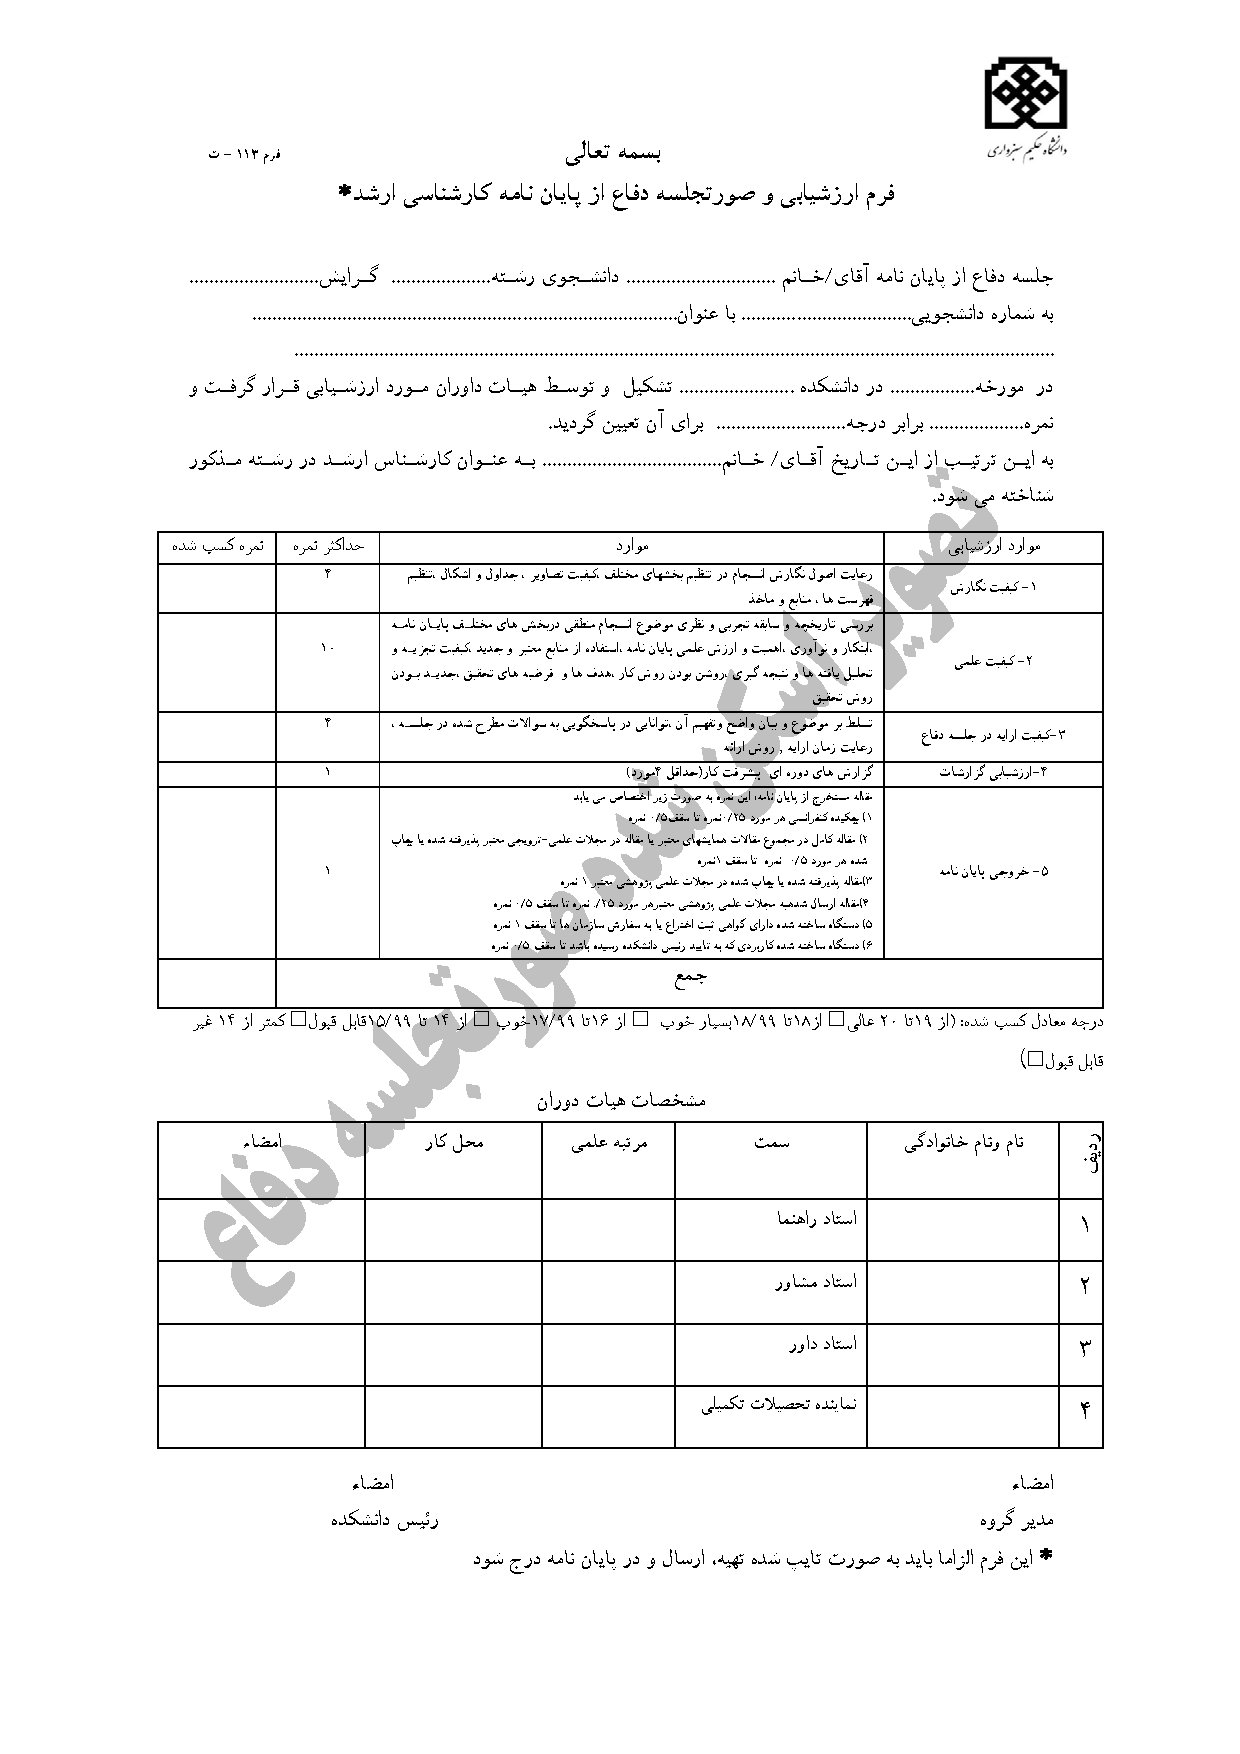
\includepdf{sooratjalaseh.pdf}

\doublespacing
\sogandPage
\esalatPage
\mojavezPage % اگر صفحه مجوز بهره برداری را نمیخواهید این خط را در حالت توضیح قرار دهید.
\sepasPage
} % end ifoptiondraft

\newpage\clearpage

\pagenumbering{alph}
\tableofcontents

\ifoptiondraft{
\setcounter{tocdepth}{1}
\listoftodos
\pagestyle{plain}
\pagenumbering{arabic}
}{%
% اگر مایلید فهرست  کلمات اختصاری را داشته باشید خط زیر را از حالت توضیح خارج کنید و کلمات خود را داخل فایل acronyms بنویسید.
%\newpage % !TEX TS-program = XeLaTeX
% !TeX root=main.tex
\chapter*{فهرست علائم اختصاری}
\addcontentsline{toc}{chapter}{فهرست علائم اختصاری}

\persiangloss{شتاب گرانش}{$a$ (m/s$^2$)}
\persiangloss{نیرو}{$F$ (N)}

\newpage \listoftables  
\newpage \listoffigures 

% اگر مایلید فهرست الگوریتمها را داشته باشید خطوط زیر را از حالت توضیح خارج کنید.
%\newpage
%\listofalgorithms 


\pagestyle{plain}
\clearpage
\pagenumbering{arabic}

\newpage
\abstractPage
}

%\setRTLparagraphfootnotes
% !TeX root=main.tex
% !TEX TS-program = XeLaTeX
\chapter*{پیش‌گفتار}
\addcontentsline{toc}{chapter}{پیش‌گفتار}

رعایت قانون‌های تدوین شده از جانب نهادهای مسؤول در دانشگاه همچون معاونت آموزشی و معاونت پژوهشی امری الزامی در حروف‌چینی مستندات علمی دانشگاهیان است. یکی از موارد پر استفاده قالب مستندات علمی، نگارش پایان‌نامه است که شامل پروژه‌های دوره کارشناسی، پایان‌نامه‌های دوره ارشد و رساله‌های دکترا می‌شود.
چارچوب کلی  نگارش \پ های دانشگاه حکیم سبزواری توسط نهادهای ذیربط مدون شده و دانشجویان این دانشگاه باید مستندات خود را بر اساس آن آماده نمایند.

پیروی از این قوانین در نرم‌افزاری مانند میکروسافت ورد
\lr{(Microsoft Word)}
  امری زمان‌بر بوده و وقت زیادی هم از دانشجو، هم استاد راهنما و هم مدیریت تحصیلات تکمیلی و کتابخانه دانشگاه در بررسی درستی کار می‌گیرد. عموماً در نهایت نیز مستندات تحویلی یک‌دست نبوده و کاملاً مطابق دستورالعمل داده شده نیستند؛ به‌این دلیل که میکروسافت ورد یک نرم‌افزار حروف‌چین نیست، بلکه یک ویرایشگر پیشرفته است.

اگر دانشجویان از یک ابزار حروف‌چینی همانند لاتک 
\lr{(\LaTeX)}
استفاده کنند، به شرطی که قالب آماده‌ای داشته باشند، لازم نیست نگران دستورالعمل داده شده باشند.
این نوشتار به بیان چنین قالب آماده‌ای برای \پ های دانشگاه حکیم سبزواری می‌پردازد که به همین منظور آماده شده است
\footnote{این قالب با حمایت معاونت پژوهشی دانشگاه حکیم سبزواری آماده شده است.}
.
در صورت استفاده از این قالب، دانشجویان هیچ کاری به دستورالعمل دانشگاه ندارند، تمامی موارد -- همچون اندازه و نوع  قلم متن و عناوین، اندازه حاشیه‌ها، صفحات آغازین و ... -- توسط کلاس آماده شده به صورت خودکار اعمال می‌گردد. دانشجویان و اساتید فقط کافیست روی محتوای کار خود تمرکز نمایند و به چگونگی حروف‌چینی هیچ کاری نخواهند داشت.
شاید دانشجویان در بدو امر مشکلاتی با یادگیری دستورات لاتک داشته باشند، اما به تدریج با یادگیری دستورات اصلی لاتک و مطالعه همین نوشتار و ملاحظه سورس آن، مشکلاتشان برطرف شده و ادامه کار برای آنها بسیار دلنشین و راحت خواهد شد.
			% پیشگفتار
%\setLTRparagraphfootnotes
% !TEX TS-program = XeLaTeX
% !TeX root=main.tex

\chapter{راهنمای استفاده از کلاس}

\section{مقدمه}
حروف‌چینی پروژه کارشناسی، پایان‌نامه یا رساله یکی از موارد پرکاربرد استفاده از زی‌پرشین\cite{Khalighi2015xepersian} است.  یک پروژه، پایان‌نامه یا رساله،  احتیاج به تنظیمات زیادی از نظر صفحه آرایی  دارد که وقت زیادی از دانشجو می گیرد.به دلیل قابلیت های بسیار لاتک در حروف‌چینی، یک کلاس با نام 
\lr{HSU-Thesis}
 برای حروف‌چینی پروژه‌ها، پایان‌نامه‌ها و رساله‌های دانشگاه حکیم سبزواری با استفاده از نرم افزار لاتک  آماده شده است. این فایل به 
گونه‌ای طراحی شده است که کلیات خواسته‌های مورد نیاز  مدیریت تحصیلات تکمیلی دانشگاه حکیم سبزواری
% \cite{IUSTThesisGuide}
 را برآورده می‌کند.% و نیز، حروف‌چینی بسیاری از قسمت‌های آن، به طور خودکار انجام می‌شود.

راهنمای نگارش پایان‌نامه دانشگاه حکیم سبزواری به دو مقوله می‌پردازد، اول قالب و چگونگی صفحه آرایی پایان‌نامه، مانند اندازه و نوع قلم بخشهای مختلف، چینش فصلها، قالب مراجع و مواردی از این قبیل و دوم محتوای هر فصل پایان‌نامه. 
درصورت استفاده از این کلاس، دانشجو  نیازی نیست که نگران مقوله اول باشد. لاتک همه کارها را برای وی انجام می دهد. فقط کافیست مطالب خود را تایپ و سند خود را با لاتک و ابزار آن اجرا کند تا پایان‌نامه خود را با قالب دانشگاه داشته باشد.
کلیه فایل‌های لازم برای حروف‌چینی با کلاس گفته شده، داخل پوشه‌ای به نام
\lr{HSU-Thesis}
  قرار داده شده است. توجه داشته باشید که برای استفاده از این کلاس باید فونت های
  \lr{IRLotusICEE}،
و
  \lr{IRTitr}
را داشته باشید (همراه با این کلاس هست و نیاز به نصب نیست).
 قلمهای 
\lr{IRLotusICEE}
  مستخرج از قلمهای
\lr{IRLotus}
شورای عالی اطلاع رسانی هستند که توسط دکتر بابایی‌زاده اصلاحاتی روی آنها صورت پذیرفته است: تبدیل صفر تو پر به صفر توخالی و اضافه شدن
\textit{\textbf{حالت توپر و ایرانیک}}،
که‌این موارد در قلمهای شورای عالی اطلاع رسانی وجود ندارد.

\section{این همه فایل؟!}\label{sec2}
از آنجایی که یک پایان‌نامه یا رساله، یک نوشته بلند محسوب می‌شود، لذا اگر همه تنظیمات و مطالب پایان‌نامه را داخل یک فایل قرار بدهیم، باعث شلوغی
و سردرگمی می‌شود. به همین خاطر، قسمت‌های مختلف پایان‌نامه یا رساله  داخل فایل‌های جداگانه قرار گرفته است. مثلاً تنظیمات پایه‌ای کلاس، داخل فایل
\lr{HSU-Thesis.cls}، 
قسمت مشخصات فارسی پایان‌نامه، داخل 
\lr{faTitle.tex}،
مطالب فصل اول، داخل 
\lr{chapter1}
و تنظیمات قابل تغییر توسط کاربر، داخل 
\lr{commands.tex}
 قرار داده شده است. 
\begin{center}
\textbf{ فایل اصلی این مجموعه، فایل
\lr{main.tex}
می‌باشد. }
\end{center}

%یعنی بعد از تغییر فایل‌های دیگر، برای دیدن نتیجه تغییرات، باید این فایل را اجرا کرد. بقیه فایل‌ها به‌این فایل، کمک می‌کنند تا بتوانیم خروجی کار را ببینیم. 
اگر به فایل 
\lr{main.tex}
دقت کنید، متوجه می شوید که قسمت‌های مختلف پایان‌نامه، توسط دستورهایی مانند 
\lr{input}
و
\lr{include}
به فایل اصلی، یعنی 
\lr{main.tex}
معرفی شده‌اند. بنابراین، فایلی که همیشه با آن سروکار داریم، فایل 
\lr{main.tex}
است.
در این فایل، فرض شده است که پایان‌نامه یا رساله شما، از دو فصل و دو پیوست، تشکیل شده است. با این حال، خودتان می‌توانید به راحتی فصل‌ها و پیوست های بیشتر را به‌این مجموعه، اضافه کنید. این کار، بسیار ساده است. فرض کنید بخواهید یک فصل دیگر هم به پایان‌نامه، اضافه کنید. برای این کار، کافی است یک فایل با نام دلخواه مثلاً 
\lr{chapter3}
و با پسوند 
\lr{.tex}
بسازید و آن را داخل پوشه 
\lr{HSU-Thesis}
قرار دهید و سپس این فایل را با دستور 
\verb!\include{chapter3}!
داخل فایل
\lr{main.tex}
 قرار دهید. توصیه می‌شود فایل 
 \lr{chapter2}
 را با نام 
 \lr{chapter3}
 ذخیره نمایید.

\section{از کجا شروع کنم؟}
قبل از هر چیز، باید یک توزیع تِک مناسب مانند تک لایو
\lr{(TeXLive)}
را روی سیستم خود نصب کنید. تک لایو  را می‌توانید از 
 \href{http://www.tug.org/texlive}{سایت رسمی آن}%
\LTRfootnote{\url{http://www.tug.org/texlive}}
 دانلود کنید یا به صورت پستی از 
 \href{http://www.parsilatex.com}{سایت پارسی‌لاتک}%
\LTRfootnote{\url{http://www.parsilatex.com}}
سفارش دهید. مورد دوم حاوی مثالهای فارسی متنوعی شامل نمونه پایان‌نامه، نمونه مقاله، جدول و ... است که کارکردن اجزای مختلف آن مورد بررسی قرار گرفته است.

برای تایپ و پردازش اسناد لاتک باید از یک ویرایشگر مناسب استفاده کنید. به همراه تک لایو ویرایشگر \lr{TeXWroks} هست که می‌توانید از آن برای پردازش اسناد خود استفاده کنید. 
ویرایش گرهای  
\lr{TeXstudio}
و
\lr{Texmaker}
امکانات بیشتری دارند که با جستجو در اینترنت می‌توانید آنها را پیدا و دانلود فرمایید. این ویرایشگرها در مجموعه‌های جدید پارسی‌لاتک نیز موجودند. به کاربران مبتدی استفاده از 
\lr{TeXstudio}
توصیه می‌شود.

 توضیحات بیشتر درخصوص چگونگی اجرای اسناد زی‌پرشین را می‌توانید در فایل راهنمای دی وی دی پارسی‌لاتک ببینید.
 
 حال اگر نوشتن \پ اولین تجربه شما از کار با لاتک است، توصیه می‌شود که یک بار به صورت اجمالی، کتاب «%
\href{http://www.tug.ctan.org/tex-archive/info/lshort/persian/lshort.pdf}{مقدمه‌ای نه چندان کوتاه بر
\lr{\LaTeXe}}»
   ترجمه دکتر مهدی امیدعلی را مطالعه کنید. این کتاب، کتاب بسیار کاملی است که خیلی از نیازهای شما در ارتباط با حروف‌چینی را برطرف می‌کند. اگر تک لایو کامل را داشته باشید، این کتاب را هم دارید. کافیست در خط فرمان دستور زیر را بزنید:
\begin{latin}
texdoc lshort-persian
\end{latin}
برای اجرای دستور از خط فرمان در ویندوز کافیست کلید ویندوز (کلید مابین کلیدهای 
\lr{Ctrl} و \lr{Alt}
) به همراه دکمه 
\lr{R}
را بفشارید و در پنجره ظاهر شده دستور فوق را بنویسد.

% در هر صورت از آدرس زیر قابل دانلود است:\\
%\lr{\url{http://www.tug.ctan.org/tex-archive/info/lshort/persian/lshort.pdf}\hfill}
اگر عجله دارید، برخی دستورات پایه‌ای مورد نیاز در فصل \ref{Chap:chapter2} بیان شده‌اند.
 
 
بعد از موارد گفته شده، فایل 
\lr{main.tex}
و
\lr{faTitle}
را باز کنید و مشخصات پایان‌نامه خود مثل نام، نام خانوادگی، عنوان پایان‌نامه و ... را جایگزین مشخصات موجود در فایل
\lr{faTitle}
 کنید. دقت داشته باشید که نیازی نیست 
نگران چینش این مشخصات در فایل پی دی اف خروجی باشید. فایل 
\lr{HSU-Thesis.cls}
همه‌این کارها را به طور خودکار برای شما انجام می دهد. در ضمن، موقع تغییر دادن دستورهای داخل فایل
\lr{faTitle}
 کاملاً دقت کنید. این دستورها، خیلی حساس هستند و ممکن است با یک تغییر کوچک، موقع اجرا، خطا بگیرید. برای دیدن خروجی کار، فایل 
\lr{faTitle}
 را 
\lr{Save}، 
(نه 
\lr{Save As})
کنید  و آن را اجرا کنید.
 فایلهای این مجموعه به گونه‌ای هستند که در \lr{TeXWorks}  یا 
\lr{TeXStudio}
بدون برگشتن به فایل اصلی، می‌توانید سند خود را اجرا کنید. 
 حال اگر می خواهید مشخصات انگلیسی \پ را هم عوض کنید، فایل 
\lr{enTitle}
را باز کنید و مشخصات داخل آن را تغییر دهید.%
%\RTLfootnote{
%برای نوشتن پروژه کارشناسی، نیازی به وارد کردن مشخصات انگلیسی پروژه نیست. بنابراین، این مشخصات، به طور خودکار،
%نادیده گرفته می‌شود.
%}
 در اینجا هم برای دیدن خروجی، باید این فایل را 
\lr{Save}
کرده و بعد به فایل 
\lr{main.tex}
برگشته و آن را اجرا کرد.

این قالب طوری طراحی شده است که کافی است فقط  یک بار مشخصات \پ  را وارد کنید. هر جای دیگر که لازم به درج این مشخصات باشد، این مشخصات به طور خودکار درج می‌شود. با این حال، اگر مایل بودید، می‌توانید تنظیمات موجود را در فایل
\lr{HSU-Thesis.cls}
  تغییر دهید. توجه داشته باشید که اگر کاربر مبتدی هستید و یا با ساختار فایل‌های  
\lr{cls}
 آشنایی ندارید، به هیچ وجه به‌این فایل دست نزنید.

نکته دیگری که باید به آن توجه کنید این است که در استیل آماده شده سه گزینه به نام‌های
\lr{bsc}،
\lr{msc}
و
\lr{phd}
برای حروف‌چینی پروژه، پایان‌نامه و رساله،
طراحی شده است. بنابراین اگر قصد تایپ پروژه کارشناسی، پایان‌نامه  ارشد یا رساله دکترا را دارید، 
 در فایل 
\lr{main.tex}
باید به ترتیب از گزینه‌های
\lr{bsc}،
\lr{msc}
و
\lr{phd}
استفاده کنید. با انتخاب هر کدام از این گزینه‌ها، تنظیمات مربوط به آنها به طور خودکار، اعمل می‌شود.    

دقت داشته باشید که شما فقط با فایلهای با پسوند 
\lr{tex} و \lr{bib}
سروکار دارید و به سایر فایلها (نظیر فایلهای
\lr{ind}، \lr{bbl}، \lr{idx} و \lr{toc}
)
نباید هیچ کاری داشته باشید. اینها فایلهای موقتی هستند که توسط لاتک تولید میشوند.
در بخش بعد فهرست فیلدهای قابل استفاده در این قالب آمده است.

%فقط برخی اطلاعات صفحه مربوط به صورتجلسه دفاع از پایان‌نامه  باید به صورت دستی وارد شوند. 

\subsection{مشخصات \پ}\label{Sec:spec}
ثبت مشخصات دانشجو و پایان‌نامه در فایل 
\lr{faTitle}
انجام می‌پذیرد. به این منظور دانشجو باید این فایل را باز نموده و مشخصات موردنظر خود را وارد نماید.
به عنوان مثال عنوان \پ در 
\verb!\title{}!
، نام استاد راهنمای اول در 
\verb!\firstadvisor{}!
و شماره دانشجویی در 
\verb!\studentID{}!
قرار می‌گیرد.

به صورت مشابه مشخصات لاتین \پ در فایل 
\lr{enTitle}
ثبت می‌شود.
دانشجو فقط یک بار اطلاعات را وارد می‌کند و قالب آماده شده، مشخصات را در جای مناسب خود قرار می‌دهد.


فهرست فیلدهای فارسی و لاتین قابل پر شدن توسط دانشجو  در جداول
\ref{faFieldList} و \ref{enFieldList}
  آمده است.
اجباری بودن یا نبودن هر فیلد در ستون سوم مشخص شده است. فیلدهای اجباری حتماً باید باشند، اما فیلدهایی که اجباری نیستند می‌توانند باشند یا نباشند.
فیلدی که قرار نیست باشد را می‌توان کلا از فایل مربوطه حذف کرد و یا با گذاشتن 
\%
آنرا به حالت توضیح درآورد.
به عنوان مثال فیلد 
\lr{secondsupervisor}
مشخص‌کننده‌ی استاد راهنمای دوم است که دانشجو می‌تواند داشته باشد یا نداشته باشد.
اگر دانشجو استاد راهنمای دوم داشته باشد و این فیلد را با برداشتن 
\%
فعال نموده و نام استاد راهنمای دوم خود را وارد کند، به صورت خودکار نام استاد راهنمای دوم در مواردی که لازم است در \پ درج خواهد شد. به علاوه در موارد موردنیاز به جای عبارت «استاد راهنما» از عبارت «استادان راهنما» استفاده خواهد شد.

همان‌گونه که در بخش قبل ذکر شد، به صورت خودکار با تغییر مقطع \پ در فایل
\lr{main}
عنوان سند به صورت خودکار اصلاح می‌شود: پروژه، پایان‌نامه و یا رساله. اما اگر عبارت دیگری به جر اینها مدنظر باشد می‌توان آنرا در فیلد
\lr{projectLabel}
مشخص کرد. همین کار برای نام دوره (کارشناسی، کارشناسی ارشد و دکترا) با فیلد
\lr{degree}
قابل انجام است.

متنهای «تقدیم به» و «سپاس‌گزاری» که با فیلدهای 
\lr{faDedication} و \lr{faAcknowledgement}
مشخص شده‌اند اختیاری هستند و هر کدام می‌توانند باشند یا نباشند.
در صورت عدم وجود هر دو، صفحه مربوطه از \پ حذف خواهد شد.

\begin{table}[h]
\centering
\caption{فهرست فیلدهای فارسی قالب پایان‌نامه که در فایل
\lr{faTitle} وجود دارند.}
\label{faFieldList}
\begin{tabular}{cccc}
\hline
 ردیف & نام فیلد & توضیح & اجباری؟\\ 
 \hline
  ۱ & \lr{university} & نام دانشگاه & بله \\ 
  ۲ & \lr{faculty} & نام دانشکده & بله \\ 
  ۳ & \lr{subject} & نام رشته & بله \\ 
  ۴ & \lr{field} & گرایش & بله \\ 
  ۵ & \lr{title} &  عنوان \پ & بله \\ 
  ۶ & \lr{firstsupervisor} & استاد راهنمای اول & بله \\ 
  ۷ & \lr{secondsupervisor} & استاد راهنمای دوم & خیر \\ 
  ۸ & \lr{firstadvisor} & مشاور اول &خیر \\ 
  ۹ & \lr{secondadvisor} & مشاور دوم &خیر \\ 
 ۱۰ & \lr{name} & نام دانشجو  & بله \\ 
 ۱۱ & \lr{surname} & نام خانوادگی دانشجو & بله \\ 
 ۱۲ & \lr{studentID} & شماره دانشجویی & بله \\ 
 ۱۳ & \lr{thesisdate} & تاریخ اتمام \پ & بله \\ 
 ۱۴ & \lr{projectLabel} & عنوان \پ & خیر \\ 
 ۱۵ & \lr{degree} & مقطع \پ & خیر \\ 
 ۱۶ & \lr{firstReviewer} & داور اول & بله \\ 
 ۱۷ & \lr{secondReviewer} & داور دوم & خیر \\ 
 ۱۸ & \lr{thirdReviewer} & داور سوم & خیر \\ 
 ۱۹ & \lr{representative} & نماینده تحصیلات تکمیلی & خیر \\ 
 ۲۰ & \lr{departmentHead} & مدیر گروه & بله \\ 
 ۲۱ & \lr{keywords} & واژگان کلیدی & بله \\ 
 ۲۲ & \lr{faAbstract} & چکیده فارسی & بله \\ 
 ۲۳ & \lr{faDedication} & متن تقدیم به & خیر \\ 
 ۲۴ & \lr{faAcknowledgement} & متن سپاس‌گزاری & خیر \\ 
\hline 
\end{tabular} 
\end{table}

\begin{table}[h]
\centering
\caption{فهرست فیلدهای انگلیسی قالب پایان‌نامه که در فایل
\lr{enTitle} وجود دارند.}
\label{enFieldList}
\begin{tabular}{cccc}
\hline
 ردیف & نام فیلد & توضیح & اجباری؟\\ 
 \hline
  ۱ & \lr{latinuniversity} & نام دانشگاه & بله \\ 
  ۲ & \lr{latinfaculty} & نام دانشکده & بله \\ 
  ۳ & \lr{latinsubject} & نام رشته & بله \\ 
  ۴ & \lr{latinfield} & گرایش & بله \\ 
  ۵ & \lr{latintitle} &  عنوان \پ & بله \\ 
  ۶ & \lr{firstlatinsupervisor} & استاد راهنمای اول & بله \\ 
  ۷ & \lr{secondlatinsupervisor} & استاد راهنمای دوم & خیر \\ 
  ۸ & \lr{firstlatinadvisor} & مشاور اول &خیر \\ 
  ۹ & \lr{secondlatinadvisor} & مشاور دوم &خیر \\ 
 ۱۰ & \lr{latinname} & نام دانشجو  & بله \\ 
 ۱۱ & \lr{latinsurname} & نام خانوادگی دانشجو & بله \\ 
 ۱۲ & \lr{latinthesisdate} & تاریخ اتمام \پ & بله \\ 
 ۱۳ & \lr{latinkeywords} & واژگان کلیدی & بله \\ 
 ۱۴ & \lr{en-abstract} & چکیده انگلیسی & بله \\ 
\hline 
\end{tabular} 
\end{table}


\section[مطالب پروژه را چطور بنویسم؟]
{مطالب \پ را چطور بنویسم؟}
\subsection{نوشتن فصل‌ها}
همان طور که در بخش \ref{sec2} گفته شد، برای جلوگیری از شلوغی و سردرگمی کاربر در هنگام حروف‌چینی، قسمت‌های مختلف \پ از جمله فصل‌ها، در فایل‌های جداگانه‌ای قرار داده شده‌اند. 

بنابراین، اگر می خواهید مثلاً مطالب فصل ۱ را تایپ کنید، باید فایل
\lr{chapter1}
را باز کنید و مطالب خود را جایگزین محتویات داخل فایل 
\lr{chapter1}
نمایید. دقت داشته باشید که در ابتدای برخی فایلها دستوراتی نوشته شده است و از شما خواسته شده است که آن دستورات را حذف نکنید.


نکته بسیار مهمی که در اینجا باید گفته شود این است که سیستم \lr{\TeX}، محتویات یک فایل تِک را به ترتیب پردازش می‌کند.  بنابراین، اگر مثلاً  دو فصل اول خود را نوشته و خروجی آنها را دیده‌اید و مشغول تایپ مطالب فصل ۳ هستید، بهتر است
که دو دستور 
\verb!% !TEX TS-program = XeLaTeX
% !TeX root=main.tex

\chapter{راهنمای استفاده از کلاس}

\section{مقدمه}
حروف‌چینی پروژه کارشناسی، پایان‌نامه یا رساله یکی از موارد پرکاربرد استفاده از زی‌پرشین\cite{Khalighi2015xepersian} است.  یک پروژه، پایان‌نامه یا رساله،  احتیاج به تنظیمات زیادی از نظر صفحه آرایی  دارد که وقت زیادی از دانشجو می گیرد.به دلیل قابلیت های بسیار لاتک در حروف‌چینی، یک کلاس با نام 
\lr{HSU-Thesis}
 برای حروف‌چینی پروژه‌ها، پایان‌نامه‌ها و رساله‌های دانشگاه حکیم سبزواری با استفاده از نرم افزار لاتک  آماده شده است. این فایل به 
گونه‌ای طراحی شده است که کلیات خواسته‌های مورد نیاز  مدیریت تحصیلات تکمیلی دانشگاه حکیم سبزواری
% \cite{IUSTThesisGuide}
 را برآورده می‌کند.% و نیز، حروف‌چینی بسیاری از قسمت‌های آن، به طور خودکار انجام می‌شود.

راهنمای نگارش پایان‌نامه دانشگاه حکیم سبزواری به دو مقوله می‌پردازد، اول قالب و چگونگی صفحه آرایی پایان‌نامه، مانند اندازه و نوع قلم بخشهای مختلف، چینش فصلها، قالب مراجع و مواردی از این قبیل و دوم محتوای هر فصل پایان‌نامه. 
درصورت استفاده از این کلاس، دانشجو  نیازی نیست که نگران مقوله اول باشد. لاتک همه کارها را برای وی انجام می دهد. فقط کافیست مطالب خود را تایپ و سند خود را با لاتک و ابزار آن اجرا کند تا پایان‌نامه خود را با قالب دانشگاه داشته باشد.
کلیه فایل‌های لازم برای حروف‌چینی با کلاس گفته شده، داخل پوشه‌ای به نام
\lr{HSU-Thesis}
  قرار داده شده است. توجه داشته باشید که برای استفاده از این کلاس باید فونت های
  \lr{IRLotusICEE}،
و
  \lr{IRTitr}
را داشته باشید (همراه با این کلاس هست و نیاز به نصب نیست).
 قلمهای 
\lr{IRLotusICEE}
  مستخرج از قلمهای
\lr{IRLotus}
شورای عالی اطلاع رسانی هستند که توسط دکتر بابایی‌زاده اصلاحاتی روی آنها صورت پذیرفته است: تبدیل صفر تو پر به صفر توخالی و اضافه شدن
\textit{\textbf{حالت توپر و ایرانیک}}،
که‌این موارد در قلمهای شورای عالی اطلاع رسانی وجود ندارد.

\section{این همه فایل؟!}\label{sec2}
از آنجایی که یک پایان‌نامه یا رساله، یک نوشته بلند محسوب می‌شود، لذا اگر همه تنظیمات و مطالب پایان‌نامه را داخل یک فایل قرار بدهیم، باعث شلوغی
و سردرگمی می‌شود. به همین خاطر، قسمت‌های مختلف پایان‌نامه یا رساله  داخل فایل‌های جداگانه قرار گرفته است. مثلاً تنظیمات پایه‌ای کلاس، داخل فایل
\lr{HSU-Thesis.cls}، 
قسمت مشخصات فارسی پایان‌نامه، داخل 
\lr{faTitle.tex}،
مطالب فصل اول، داخل 
\lr{chapter1}
و تنظیمات قابل تغییر توسط کاربر، داخل 
\lr{commands.tex}
 قرار داده شده است. 
\begin{center}
\textbf{ فایل اصلی این مجموعه، فایل
\lr{main.tex}
می‌باشد. }
\end{center}

%یعنی بعد از تغییر فایل‌های دیگر، برای دیدن نتیجه تغییرات، باید این فایل را اجرا کرد. بقیه فایل‌ها به‌این فایل، کمک می‌کنند تا بتوانیم خروجی کار را ببینیم. 
اگر به فایل 
\lr{main.tex}
دقت کنید، متوجه می شوید که قسمت‌های مختلف پایان‌نامه، توسط دستورهایی مانند 
\lr{input}
و
\lr{include}
به فایل اصلی، یعنی 
\lr{main.tex}
معرفی شده‌اند. بنابراین، فایلی که همیشه با آن سروکار داریم، فایل 
\lr{main.tex}
است.
در این فایل، فرض شده است که پایان‌نامه یا رساله شما، از دو فصل و دو پیوست، تشکیل شده است. با این حال، خودتان می‌توانید به راحتی فصل‌ها و پیوست های بیشتر را به‌این مجموعه، اضافه کنید. این کار، بسیار ساده است. فرض کنید بخواهید یک فصل دیگر هم به پایان‌نامه، اضافه کنید. برای این کار، کافی است یک فایل با نام دلخواه مثلاً 
\lr{chapter3}
و با پسوند 
\lr{.tex}
بسازید و آن را داخل پوشه 
\lr{HSU-Thesis}
قرار دهید و سپس این فایل را با دستور 
\verb!\include{chapter3}!
داخل فایل
\lr{main.tex}
 قرار دهید. توصیه می‌شود فایل 
 \lr{chapter2}
 را با نام 
 \lr{chapter3}
 ذخیره نمایید.

\section{از کجا شروع کنم؟}
قبل از هر چیز، باید یک توزیع تِک مناسب مانند تک لایو
\lr{(TeXLive)}
را روی سیستم خود نصب کنید. تک لایو  را می‌توانید از 
 \href{http://www.tug.org/texlive}{سایت رسمی آن}%
\LTRfootnote{\url{http://www.tug.org/texlive}}
 دانلود کنید یا به صورت پستی از 
 \href{http://www.parsilatex.com}{سایت پارسی‌لاتک}%
\LTRfootnote{\url{http://www.parsilatex.com}}
سفارش دهید. مورد دوم حاوی مثالهای فارسی متنوعی شامل نمونه پایان‌نامه، نمونه مقاله، جدول و ... است که کارکردن اجزای مختلف آن مورد بررسی قرار گرفته است.

برای تایپ و پردازش اسناد لاتک باید از یک ویرایشگر مناسب استفاده کنید. به همراه تک لایو ویرایشگر \lr{TeXWroks} هست که می‌توانید از آن برای پردازش اسناد خود استفاده کنید. 
ویرایش گرهای  
\lr{TeXstudio}
و
\lr{Texmaker}
امکانات بیشتری دارند که با جستجو در اینترنت می‌توانید آنها را پیدا و دانلود فرمایید. این ویرایشگرها در مجموعه‌های جدید پارسی‌لاتک نیز موجودند. به کاربران مبتدی استفاده از 
\lr{TeXstudio}
توصیه می‌شود.

 توضیحات بیشتر درخصوص چگونگی اجرای اسناد زی‌پرشین را می‌توانید در فایل راهنمای دی وی دی پارسی‌لاتک ببینید.
 
 حال اگر نوشتن \پ اولین تجربه شما از کار با لاتک است، توصیه می‌شود که یک بار به صورت اجمالی، کتاب «%
\href{http://www.tug.ctan.org/tex-archive/info/lshort/persian/lshort.pdf}{مقدمه‌ای نه چندان کوتاه بر
\lr{\LaTeXe}}»
   ترجمه دکتر مهدی امیدعلی را مطالعه کنید. این کتاب، کتاب بسیار کاملی است که خیلی از نیازهای شما در ارتباط با حروف‌چینی را برطرف می‌کند. اگر تک لایو کامل را داشته باشید، این کتاب را هم دارید. کافیست در خط فرمان دستور زیر را بزنید:
\begin{latin}
texdoc lshort-persian
\end{latin}
برای اجرای دستور از خط فرمان در ویندوز کافیست کلید ویندوز (کلید مابین کلیدهای 
\lr{Ctrl} و \lr{Alt}
) به همراه دکمه 
\lr{R}
را بفشارید و در پنجره ظاهر شده دستور فوق را بنویسد.

% در هر صورت از آدرس زیر قابل دانلود است:\\
%\lr{\url{http://www.tug.ctan.org/tex-archive/info/lshort/persian/lshort.pdf}\hfill}
اگر عجله دارید، برخی دستورات پایه‌ای مورد نیاز در فصل \ref{Chap:chapter2} بیان شده‌اند.
 
 
بعد از موارد گفته شده، فایل 
\lr{main.tex}
و
\lr{faTitle}
را باز کنید و مشخصات پایان‌نامه خود مثل نام، نام خانوادگی، عنوان پایان‌نامه و ... را جایگزین مشخصات موجود در فایل
\lr{faTitle}
 کنید. دقت داشته باشید که نیازی نیست 
نگران چینش این مشخصات در فایل پی دی اف خروجی باشید. فایل 
\lr{HSU-Thesis.cls}
همه‌این کارها را به طور خودکار برای شما انجام می دهد. در ضمن، موقع تغییر دادن دستورهای داخل فایل
\lr{faTitle}
 کاملاً دقت کنید. این دستورها، خیلی حساس هستند و ممکن است با یک تغییر کوچک، موقع اجرا، خطا بگیرید. برای دیدن خروجی کار، فایل 
\lr{faTitle}
 را 
\lr{Save}، 
(نه 
\lr{Save As})
کنید  و آن را اجرا کنید.
 فایلهای این مجموعه به گونه‌ای هستند که در \lr{TeXWorks}  یا 
\lr{TeXStudio}
بدون برگشتن به فایل اصلی، می‌توانید سند خود را اجرا کنید. 
 حال اگر می خواهید مشخصات انگلیسی \پ را هم عوض کنید، فایل 
\lr{enTitle}
را باز کنید و مشخصات داخل آن را تغییر دهید.%
%\RTLfootnote{
%برای نوشتن پروژه کارشناسی، نیازی به وارد کردن مشخصات انگلیسی پروژه نیست. بنابراین، این مشخصات، به طور خودکار،
%نادیده گرفته می‌شود.
%}
 در اینجا هم برای دیدن خروجی، باید این فایل را 
\lr{Save}
کرده و بعد به فایل 
\lr{main.tex}
برگشته و آن را اجرا کرد.

این قالب طوری طراحی شده است که کافی است فقط  یک بار مشخصات \پ  را وارد کنید. هر جای دیگر که لازم به درج این مشخصات باشد، این مشخصات به طور خودکار درج می‌شود. با این حال، اگر مایل بودید، می‌توانید تنظیمات موجود را در فایل
\lr{HSU-Thesis.cls}
  تغییر دهید. توجه داشته باشید که اگر کاربر مبتدی هستید و یا با ساختار فایل‌های  
\lr{cls}
 آشنایی ندارید، به هیچ وجه به‌این فایل دست نزنید.

نکته دیگری که باید به آن توجه کنید این است که در استیل آماده شده سه گزینه به نام‌های
\lr{bsc}،
\lr{msc}
و
\lr{phd}
برای حروف‌چینی پروژه، پایان‌نامه و رساله،
طراحی شده است. بنابراین اگر قصد تایپ پروژه کارشناسی، پایان‌نامه  ارشد یا رساله دکترا را دارید، 
 در فایل 
\lr{main.tex}
باید به ترتیب از گزینه‌های
\lr{bsc}،
\lr{msc}
و
\lr{phd}
استفاده کنید. با انتخاب هر کدام از این گزینه‌ها، تنظیمات مربوط به آنها به طور خودکار، اعمل می‌شود.    

دقت داشته باشید که شما فقط با فایلهای با پسوند 
\lr{tex} و \lr{bib}
سروکار دارید و به سایر فایلها (نظیر فایلهای
\lr{ind}، \lr{bbl}، \lr{idx} و \lr{toc}
)
نباید هیچ کاری داشته باشید. اینها فایلهای موقتی هستند که توسط لاتک تولید میشوند.
در بخش بعد فهرست فیلدهای قابل استفاده در این قالب آمده است.

%فقط برخی اطلاعات صفحه مربوط به صورتجلسه دفاع از پایان‌نامه  باید به صورت دستی وارد شوند. 

\subsection{مشخصات \پ}\label{Sec:spec}
ثبت مشخصات دانشجو و پایان‌نامه در فایل 
\lr{faTitle}
انجام می‌پذیرد. به این منظور دانشجو باید این فایل را باز نموده و مشخصات موردنظر خود را وارد نماید.
به عنوان مثال عنوان \پ در 
\verb!\title{}!
، نام استاد راهنمای اول در 
\verb!\firstadvisor{}!
و شماره دانشجویی در 
\verb!\studentID{}!
قرار می‌گیرد.

به صورت مشابه مشخصات لاتین \پ در فایل 
\lr{enTitle}
ثبت می‌شود.
دانشجو فقط یک بار اطلاعات را وارد می‌کند و قالب آماده شده، مشخصات را در جای مناسب خود قرار می‌دهد.


فهرست فیلدهای فارسی و لاتین قابل پر شدن توسط دانشجو  در جداول
\ref{faFieldList} و \ref{enFieldList}
  آمده است.
اجباری بودن یا نبودن هر فیلد در ستون سوم مشخص شده است. فیلدهای اجباری حتماً باید باشند، اما فیلدهایی که اجباری نیستند می‌توانند باشند یا نباشند.
فیلدی که قرار نیست باشد را می‌توان کلا از فایل مربوطه حذف کرد و یا با گذاشتن 
\%
آنرا به حالت توضیح درآورد.
به عنوان مثال فیلد 
\lr{secondsupervisor}
مشخص‌کننده‌ی استاد راهنمای دوم است که دانشجو می‌تواند داشته باشد یا نداشته باشد.
اگر دانشجو استاد راهنمای دوم داشته باشد و این فیلد را با برداشتن 
\%
فعال نموده و نام استاد راهنمای دوم خود را وارد کند، به صورت خودکار نام استاد راهنمای دوم در مواردی که لازم است در \پ درج خواهد شد. به علاوه در موارد موردنیاز به جای عبارت «استاد راهنما» از عبارت «استادان راهنما» استفاده خواهد شد.

همان‌گونه که در بخش قبل ذکر شد، به صورت خودکار با تغییر مقطع \پ در فایل
\lr{main}
عنوان سند به صورت خودکار اصلاح می‌شود: پروژه، پایان‌نامه و یا رساله. اما اگر عبارت دیگری به جر اینها مدنظر باشد می‌توان آنرا در فیلد
\lr{projectLabel}
مشخص کرد. همین کار برای نام دوره (کارشناسی، کارشناسی ارشد و دکترا) با فیلد
\lr{degree}
قابل انجام است.

متنهای «تقدیم به» و «سپاس‌گزاری» که با فیلدهای 
\lr{faDedication} و \lr{faAcknowledgement}
مشخص شده‌اند اختیاری هستند و هر کدام می‌توانند باشند یا نباشند.
در صورت عدم وجود هر دو، صفحه مربوطه از \پ حذف خواهد شد.

\begin{table}[h]
\centering
\caption{فهرست فیلدهای فارسی قالب پایان‌نامه که در فایل
\lr{faTitle} وجود دارند.}
\label{faFieldList}
\begin{tabular}{cccc}
\hline
 ردیف & نام فیلد & توضیح & اجباری؟\\ 
 \hline
  ۱ & \lr{university} & نام دانشگاه & بله \\ 
  ۲ & \lr{faculty} & نام دانشکده & بله \\ 
  ۳ & \lr{subject} & نام رشته & بله \\ 
  ۴ & \lr{field} & گرایش & بله \\ 
  ۵ & \lr{title} &  عنوان \پ & بله \\ 
  ۶ & \lr{firstsupervisor} & استاد راهنمای اول & بله \\ 
  ۷ & \lr{secondsupervisor} & استاد راهنمای دوم & خیر \\ 
  ۸ & \lr{firstadvisor} & مشاور اول &خیر \\ 
  ۹ & \lr{secondadvisor} & مشاور دوم &خیر \\ 
 ۱۰ & \lr{name} & نام دانشجو  & بله \\ 
 ۱۱ & \lr{surname} & نام خانوادگی دانشجو & بله \\ 
 ۱۲ & \lr{studentID} & شماره دانشجویی & بله \\ 
 ۱۳ & \lr{thesisdate} & تاریخ اتمام \پ & بله \\ 
 ۱۴ & \lr{projectLabel} & عنوان \پ & خیر \\ 
 ۱۵ & \lr{degree} & مقطع \پ & خیر \\ 
 ۱۶ & \lr{firstReviewer} & داور اول & بله \\ 
 ۱۷ & \lr{secondReviewer} & داور دوم & خیر \\ 
 ۱۸ & \lr{thirdReviewer} & داور سوم & خیر \\ 
 ۱۹ & \lr{representative} & نماینده تحصیلات تکمیلی & خیر \\ 
 ۲۰ & \lr{departmentHead} & مدیر گروه & بله \\ 
 ۲۱ & \lr{keywords} & واژگان کلیدی & بله \\ 
 ۲۲ & \lr{faAbstract} & چکیده فارسی & بله \\ 
 ۲۳ & \lr{faDedication} & متن تقدیم به & خیر \\ 
 ۲۴ & \lr{faAcknowledgement} & متن سپاس‌گزاری & خیر \\ 
\hline 
\end{tabular} 
\end{table}

\begin{table}[h]
\centering
\caption{فهرست فیلدهای انگلیسی قالب پایان‌نامه که در فایل
\lr{enTitle} وجود دارند.}
\label{enFieldList}
\begin{tabular}{cccc}
\hline
 ردیف & نام فیلد & توضیح & اجباری؟\\ 
 \hline
  ۱ & \lr{latinuniversity} & نام دانشگاه & بله \\ 
  ۲ & \lr{latinfaculty} & نام دانشکده & بله \\ 
  ۳ & \lr{latinsubject} & نام رشته & بله \\ 
  ۴ & \lr{latinfield} & گرایش & بله \\ 
  ۵ & \lr{latintitle} &  عنوان \پ & بله \\ 
  ۶ & \lr{firstlatinsupervisor} & استاد راهنمای اول & بله \\ 
  ۷ & \lr{secondlatinsupervisor} & استاد راهنمای دوم & خیر \\ 
  ۸ & \lr{firstlatinadvisor} & مشاور اول &خیر \\ 
  ۹ & \lr{secondlatinadvisor} & مشاور دوم &خیر \\ 
 ۱۰ & \lr{latinname} & نام دانشجو  & بله \\ 
 ۱۱ & \lr{latinsurname} & نام خانوادگی دانشجو & بله \\ 
 ۱۲ & \lr{latinthesisdate} & تاریخ اتمام \پ & بله \\ 
 ۱۳ & \lr{latinkeywords} & واژگان کلیدی & بله \\ 
 ۱۴ & \lr{en-abstract} & چکیده انگلیسی & بله \\ 
\hline 
\end{tabular} 
\end{table}


\section[مطالب پروژه را چطور بنویسم؟]
{مطالب \پ را چطور بنویسم؟}
\subsection{نوشتن فصل‌ها}
همان طور که در بخش \ref{sec2} گفته شد، برای جلوگیری از شلوغی و سردرگمی کاربر در هنگام حروف‌چینی، قسمت‌های مختلف \پ از جمله فصل‌ها، در فایل‌های جداگانه‌ای قرار داده شده‌اند. 

بنابراین، اگر می خواهید مثلاً مطالب فصل ۱ را تایپ کنید، باید فایل
\lr{chapter1}
را باز کنید و مطالب خود را جایگزین محتویات داخل فایل 
\lr{chapter1}
نمایید. دقت داشته باشید که در ابتدای برخی فایلها دستوراتی نوشته شده است و از شما خواسته شده است که آن دستورات را حذف نکنید.


نکته بسیار مهمی که در اینجا باید گفته شود این است که سیستم \lr{\TeX}، محتویات یک فایل تِک را به ترتیب پردازش می‌کند.  بنابراین، اگر مثلاً  دو فصل اول خود را نوشته و خروجی آنها را دیده‌اید و مشغول تایپ مطالب فصل ۳ هستید، بهتر است
که دو دستور 
\verb!% !TEX TS-program = XeLaTeX
% !TeX root=main.tex

\chapter{راهنمای استفاده از کلاس}

\section{مقدمه}
حروف‌چینی پروژه کارشناسی، پایان‌نامه یا رساله یکی از موارد پرکاربرد استفاده از زی‌پرشین\cite{Khalighi2015xepersian} است.  یک پروژه، پایان‌نامه یا رساله،  احتیاج به تنظیمات زیادی از نظر صفحه آرایی  دارد که وقت زیادی از دانشجو می گیرد.به دلیل قابلیت های بسیار لاتک در حروف‌چینی، یک کلاس با نام 
\lr{HSU-Thesis}
 برای حروف‌چینی پروژه‌ها، پایان‌نامه‌ها و رساله‌های دانشگاه حکیم سبزواری با استفاده از نرم افزار لاتک  آماده شده است. این فایل به 
گونه‌ای طراحی شده است که کلیات خواسته‌های مورد نیاز  مدیریت تحصیلات تکمیلی دانشگاه حکیم سبزواری
% \cite{IUSTThesisGuide}
 را برآورده می‌کند.% و نیز، حروف‌چینی بسیاری از قسمت‌های آن، به طور خودکار انجام می‌شود.

راهنمای نگارش پایان‌نامه دانشگاه حکیم سبزواری به دو مقوله می‌پردازد، اول قالب و چگونگی صفحه آرایی پایان‌نامه، مانند اندازه و نوع قلم بخشهای مختلف، چینش فصلها، قالب مراجع و مواردی از این قبیل و دوم محتوای هر فصل پایان‌نامه. 
درصورت استفاده از این کلاس، دانشجو  نیازی نیست که نگران مقوله اول باشد. لاتک همه کارها را برای وی انجام می دهد. فقط کافیست مطالب خود را تایپ و سند خود را با لاتک و ابزار آن اجرا کند تا پایان‌نامه خود را با قالب دانشگاه داشته باشد.
کلیه فایل‌های لازم برای حروف‌چینی با کلاس گفته شده، داخل پوشه‌ای به نام
\lr{HSU-Thesis}
  قرار داده شده است. توجه داشته باشید که برای استفاده از این کلاس باید فونت های
  \lr{IRLotusICEE}،
و
  \lr{IRTitr}
را داشته باشید (همراه با این کلاس هست و نیاز به نصب نیست).
 قلمهای 
\lr{IRLotusICEE}
  مستخرج از قلمهای
\lr{IRLotus}
شورای عالی اطلاع رسانی هستند که توسط دکتر بابایی‌زاده اصلاحاتی روی آنها صورت پذیرفته است: تبدیل صفر تو پر به صفر توخالی و اضافه شدن
\textit{\textbf{حالت توپر و ایرانیک}}،
که‌این موارد در قلمهای شورای عالی اطلاع رسانی وجود ندارد.

\section{این همه فایل؟!}\label{sec2}
از آنجایی که یک پایان‌نامه یا رساله، یک نوشته بلند محسوب می‌شود، لذا اگر همه تنظیمات و مطالب پایان‌نامه را داخل یک فایل قرار بدهیم، باعث شلوغی
و سردرگمی می‌شود. به همین خاطر، قسمت‌های مختلف پایان‌نامه یا رساله  داخل فایل‌های جداگانه قرار گرفته است. مثلاً تنظیمات پایه‌ای کلاس، داخل فایل
\lr{HSU-Thesis.cls}، 
قسمت مشخصات فارسی پایان‌نامه، داخل 
\lr{faTitle.tex}،
مطالب فصل اول، داخل 
\lr{chapter1}
و تنظیمات قابل تغییر توسط کاربر، داخل 
\lr{commands.tex}
 قرار داده شده است. 
\begin{center}
\textbf{ فایل اصلی این مجموعه، فایل
\lr{main.tex}
می‌باشد. }
\end{center}

%یعنی بعد از تغییر فایل‌های دیگر، برای دیدن نتیجه تغییرات، باید این فایل را اجرا کرد. بقیه فایل‌ها به‌این فایل، کمک می‌کنند تا بتوانیم خروجی کار را ببینیم. 
اگر به فایل 
\lr{main.tex}
دقت کنید، متوجه می شوید که قسمت‌های مختلف پایان‌نامه، توسط دستورهایی مانند 
\lr{input}
و
\lr{include}
به فایل اصلی، یعنی 
\lr{main.tex}
معرفی شده‌اند. بنابراین، فایلی که همیشه با آن سروکار داریم، فایل 
\lr{main.tex}
است.
در این فایل، فرض شده است که پایان‌نامه یا رساله شما، از دو فصل و دو پیوست، تشکیل شده است. با این حال، خودتان می‌توانید به راحتی فصل‌ها و پیوست های بیشتر را به‌این مجموعه، اضافه کنید. این کار، بسیار ساده است. فرض کنید بخواهید یک فصل دیگر هم به پایان‌نامه، اضافه کنید. برای این کار، کافی است یک فایل با نام دلخواه مثلاً 
\lr{chapter3}
و با پسوند 
\lr{.tex}
بسازید و آن را داخل پوشه 
\lr{HSU-Thesis}
قرار دهید و سپس این فایل را با دستور 
\verb!\include{chapter3}!
داخل فایل
\lr{main.tex}
 قرار دهید. توصیه می‌شود فایل 
 \lr{chapter2}
 را با نام 
 \lr{chapter3}
 ذخیره نمایید.

\section{از کجا شروع کنم؟}
قبل از هر چیز، باید یک توزیع تِک مناسب مانند تک لایو
\lr{(TeXLive)}
را روی سیستم خود نصب کنید. تک لایو  را می‌توانید از 
 \href{http://www.tug.org/texlive}{سایت رسمی آن}%
\LTRfootnote{\url{http://www.tug.org/texlive}}
 دانلود کنید یا به صورت پستی از 
 \href{http://www.parsilatex.com}{سایت پارسی‌لاتک}%
\LTRfootnote{\url{http://www.parsilatex.com}}
سفارش دهید. مورد دوم حاوی مثالهای فارسی متنوعی شامل نمونه پایان‌نامه، نمونه مقاله، جدول و ... است که کارکردن اجزای مختلف آن مورد بررسی قرار گرفته است.

برای تایپ و پردازش اسناد لاتک باید از یک ویرایشگر مناسب استفاده کنید. به همراه تک لایو ویرایشگر \lr{TeXWroks} هست که می‌توانید از آن برای پردازش اسناد خود استفاده کنید. 
ویرایش گرهای  
\lr{TeXstudio}
و
\lr{Texmaker}
امکانات بیشتری دارند که با جستجو در اینترنت می‌توانید آنها را پیدا و دانلود فرمایید. این ویرایشگرها در مجموعه‌های جدید پارسی‌لاتک نیز موجودند. به کاربران مبتدی استفاده از 
\lr{TeXstudio}
توصیه می‌شود.

 توضیحات بیشتر درخصوص چگونگی اجرای اسناد زی‌پرشین را می‌توانید در فایل راهنمای دی وی دی پارسی‌لاتک ببینید.
 
 حال اگر نوشتن \پ اولین تجربه شما از کار با لاتک است، توصیه می‌شود که یک بار به صورت اجمالی، کتاب «%
\href{http://www.tug.ctan.org/tex-archive/info/lshort/persian/lshort.pdf}{مقدمه‌ای نه چندان کوتاه بر
\lr{\LaTeXe}}»
   ترجمه دکتر مهدی امیدعلی را مطالعه کنید. این کتاب، کتاب بسیار کاملی است که خیلی از نیازهای شما در ارتباط با حروف‌چینی را برطرف می‌کند. اگر تک لایو کامل را داشته باشید، این کتاب را هم دارید. کافیست در خط فرمان دستور زیر را بزنید:
\begin{latin}
texdoc lshort-persian
\end{latin}
برای اجرای دستور از خط فرمان در ویندوز کافیست کلید ویندوز (کلید مابین کلیدهای 
\lr{Ctrl} و \lr{Alt}
) به همراه دکمه 
\lr{R}
را بفشارید و در پنجره ظاهر شده دستور فوق را بنویسد.

% در هر صورت از آدرس زیر قابل دانلود است:\\
%\lr{\url{http://www.tug.ctan.org/tex-archive/info/lshort/persian/lshort.pdf}\hfill}
اگر عجله دارید، برخی دستورات پایه‌ای مورد نیاز در فصل \ref{Chap:chapter2} بیان شده‌اند.
 
 
بعد از موارد گفته شده، فایل 
\lr{main.tex}
و
\lr{faTitle}
را باز کنید و مشخصات پایان‌نامه خود مثل نام، نام خانوادگی، عنوان پایان‌نامه و ... را جایگزین مشخصات موجود در فایل
\lr{faTitle}
 کنید. دقت داشته باشید که نیازی نیست 
نگران چینش این مشخصات در فایل پی دی اف خروجی باشید. فایل 
\lr{HSU-Thesis.cls}
همه‌این کارها را به طور خودکار برای شما انجام می دهد. در ضمن، موقع تغییر دادن دستورهای داخل فایل
\lr{faTitle}
 کاملاً دقت کنید. این دستورها، خیلی حساس هستند و ممکن است با یک تغییر کوچک، موقع اجرا، خطا بگیرید. برای دیدن خروجی کار، فایل 
\lr{faTitle}
 را 
\lr{Save}، 
(نه 
\lr{Save As})
کنید  و آن را اجرا کنید.
 فایلهای این مجموعه به گونه‌ای هستند که در \lr{TeXWorks}  یا 
\lr{TeXStudio}
بدون برگشتن به فایل اصلی، می‌توانید سند خود را اجرا کنید. 
 حال اگر می خواهید مشخصات انگلیسی \پ را هم عوض کنید، فایل 
\lr{enTitle}
را باز کنید و مشخصات داخل آن را تغییر دهید.%
%\RTLfootnote{
%برای نوشتن پروژه کارشناسی، نیازی به وارد کردن مشخصات انگلیسی پروژه نیست. بنابراین، این مشخصات، به طور خودکار،
%نادیده گرفته می‌شود.
%}
 در اینجا هم برای دیدن خروجی، باید این فایل را 
\lr{Save}
کرده و بعد به فایل 
\lr{main.tex}
برگشته و آن را اجرا کرد.

این قالب طوری طراحی شده است که کافی است فقط  یک بار مشخصات \پ  را وارد کنید. هر جای دیگر که لازم به درج این مشخصات باشد، این مشخصات به طور خودکار درج می‌شود. با این حال، اگر مایل بودید، می‌توانید تنظیمات موجود را در فایل
\lr{HSU-Thesis.cls}
  تغییر دهید. توجه داشته باشید که اگر کاربر مبتدی هستید و یا با ساختار فایل‌های  
\lr{cls}
 آشنایی ندارید، به هیچ وجه به‌این فایل دست نزنید.

نکته دیگری که باید به آن توجه کنید این است که در استیل آماده شده سه گزینه به نام‌های
\lr{bsc}،
\lr{msc}
و
\lr{phd}
برای حروف‌چینی پروژه، پایان‌نامه و رساله،
طراحی شده است. بنابراین اگر قصد تایپ پروژه کارشناسی، پایان‌نامه  ارشد یا رساله دکترا را دارید، 
 در فایل 
\lr{main.tex}
باید به ترتیب از گزینه‌های
\lr{bsc}،
\lr{msc}
و
\lr{phd}
استفاده کنید. با انتخاب هر کدام از این گزینه‌ها، تنظیمات مربوط به آنها به طور خودکار، اعمل می‌شود.    

دقت داشته باشید که شما فقط با فایلهای با پسوند 
\lr{tex} و \lr{bib}
سروکار دارید و به سایر فایلها (نظیر فایلهای
\lr{ind}، \lr{bbl}، \lr{idx} و \lr{toc}
)
نباید هیچ کاری داشته باشید. اینها فایلهای موقتی هستند که توسط لاتک تولید میشوند.
در بخش بعد فهرست فیلدهای قابل استفاده در این قالب آمده است.

%فقط برخی اطلاعات صفحه مربوط به صورتجلسه دفاع از پایان‌نامه  باید به صورت دستی وارد شوند. 

\subsection{مشخصات \پ}\label{Sec:spec}
ثبت مشخصات دانشجو و پایان‌نامه در فایل 
\lr{faTitle}
انجام می‌پذیرد. به این منظور دانشجو باید این فایل را باز نموده و مشخصات موردنظر خود را وارد نماید.
به عنوان مثال عنوان \پ در 
\verb!\title{}!
، نام استاد راهنمای اول در 
\verb!\firstadvisor{}!
و شماره دانشجویی در 
\verb!\studentID{}!
قرار می‌گیرد.

به صورت مشابه مشخصات لاتین \پ در فایل 
\lr{enTitle}
ثبت می‌شود.
دانشجو فقط یک بار اطلاعات را وارد می‌کند و قالب آماده شده، مشخصات را در جای مناسب خود قرار می‌دهد.


فهرست فیلدهای فارسی و لاتین قابل پر شدن توسط دانشجو  در جداول
\ref{faFieldList} و \ref{enFieldList}
  آمده است.
اجباری بودن یا نبودن هر فیلد در ستون سوم مشخص شده است. فیلدهای اجباری حتماً باید باشند، اما فیلدهایی که اجباری نیستند می‌توانند باشند یا نباشند.
فیلدی که قرار نیست باشد را می‌توان کلا از فایل مربوطه حذف کرد و یا با گذاشتن 
\%
آنرا به حالت توضیح درآورد.
به عنوان مثال فیلد 
\lr{secondsupervisor}
مشخص‌کننده‌ی استاد راهنمای دوم است که دانشجو می‌تواند داشته باشد یا نداشته باشد.
اگر دانشجو استاد راهنمای دوم داشته باشد و این فیلد را با برداشتن 
\%
فعال نموده و نام استاد راهنمای دوم خود را وارد کند، به صورت خودکار نام استاد راهنمای دوم در مواردی که لازم است در \پ درج خواهد شد. به علاوه در موارد موردنیاز به جای عبارت «استاد راهنما» از عبارت «استادان راهنما» استفاده خواهد شد.

همان‌گونه که در بخش قبل ذکر شد، به صورت خودکار با تغییر مقطع \پ در فایل
\lr{main}
عنوان سند به صورت خودکار اصلاح می‌شود: پروژه، پایان‌نامه و یا رساله. اما اگر عبارت دیگری به جر اینها مدنظر باشد می‌توان آنرا در فیلد
\lr{projectLabel}
مشخص کرد. همین کار برای نام دوره (کارشناسی، کارشناسی ارشد و دکترا) با فیلد
\lr{degree}
قابل انجام است.

متنهای «تقدیم به» و «سپاس‌گزاری» که با فیلدهای 
\lr{faDedication} و \lr{faAcknowledgement}
مشخص شده‌اند اختیاری هستند و هر کدام می‌توانند باشند یا نباشند.
در صورت عدم وجود هر دو، صفحه مربوطه از \پ حذف خواهد شد.

\begin{table}[h]
\centering
\caption{فهرست فیلدهای فارسی قالب پایان‌نامه که در فایل
\lr{faTitle} وجود دارند.}
\label{faFieldList}
\begin{tabular}{cccc}
\hline
 ردیف & نام فیلد & توضیح & اجباری؟\\ 
 \hline
  ۱ & \lr{university} & نام دانشگاه & بله \\ 
  ۲ & \lr{faculty} & نام دانشکده & بله \\ 
  ۳ & \lr{subject} & نام رشته & بله \\ 
  ۴ & \lr{field} & گرایش & بله \\ 
  ۵ & \lr{title} &  عنوان \پ & بله \\ 
  ۶ & \lr{firstsupervisor} & استاد راهنمای اول & بله \\ 
  ۷ & \lr{secondsupervisor} & استاد راهنمای دوم & خیر \\ 
  ۸ & \lr{firstadvisor} & مشاور اول &خیر \\ 
  ۹ & \lr{secondadvisor} & مشاور دوم &خیر \\ 
 ۱۰ & \lr{name} & نام دانشجو  & بله \\ 
 ۱۱ & \lr{surname} & نام خانوادگی دانشجو & بله \\ 
 ۱۲ & \lr{studentID} & شماره دانشجویی & بله \\ 
 ۱۳ & \lr{thesisdate} & تاریخ اتمام \پ & بله \\ 
 ۱۴ & \lr{projectLabel} & عنوان \پ & خیر \\ 
 ۱۵ & \lr{degree} & مقطع \پ & خیر \\ 
 ۱۶ & \lr{firstReviewer} & داور اول & بله \\ 
 ۱۷ & \lr{secondReviewer} & داور دوم & خیر \\ 
 ۱۸ & \lr{thirdReviewer} & داور سوم & خیر \\ 
 ۱۹ & \lr{representative} & نماینده تحصیلات تکمیلی & خیر \\ 
 ۲۰ & \lr{departmentHead} & مدیر گروه & بله \\ 
 ۲۱ & \lr{keywords} & واژگان کلیدی & بله \\ 
 ۲۲ & \lr{faAbstract} & چکیده فارسی & بله \\ 
 ۲۳ & \lr{faDedication} & متن تقدیم به & خیر \\ 
 ۲۴ & \lr{faAcknowledgement} & متن سپاس‌گزاری & خیر \\ 
\hline 
\end{tabular} 
\end{table}

\begin{table}[h]
\centering
\caption{فهرست فیلدهای انگلیسی قالب پایان‌نامه که در فایل
\lr{enTitle} وجود دارند.}
\label{enFieldList}
\begin{tabular}{cccc}
\hline
 ردیف & نام فیلد & توضیح & اجباری؟\\ 
 \hline
  ۱ & \lr{latinuniversity} & نام دانشگاه & بله \\ 
  ۲ & \lr{latinfaculty} & نام دانشکده & بله \\ 
  ۳ & \lr{latinsubject} & نام رشته & بله \\ 
  ۴ & \lr{latinfield} & گرایش & بله \\ 
  ۵ & \lr{latintitle} &  عنوان \پ & بله \\ 
  ۶ & \lr{firstlatinsupervisor} & استاد راهنمای اول & بله \\ 
  ۷ & \lr{secondlatinsupervisor} & استاد راهنمای دوم & خیر \\ 
  ۸ & \lr{firstlatinadvisor} & مشاور اول &خیر \\ 
  ۹ & \lr{secondlatinadvisor} & مشاور دوم &خیر \\ 
 ۱۰ & \lr{latinname} & نام دانشجو  & بله \\ 
 ۱۱ & \lr{latinsurname} & نام خانوادگی دانشجو & بله \\ 
 ۱۲ & \lr{latinthesisdate} & تاریخ اتمام \پ & بله \\ 
 ۱۳ & \lr{latinkeywords} & واژگان کلیدی & بله \\ 
 ۱۴ & \lr{en-abstract} & چکیده انگلیسی & بله \\ 
\hline 
\end{tabular} 
\end{table}


\section[مطالب پروژه را چطور بنویسم؟]
{مطالب \پ را چطور بنویسم؟}
\subsection{نوشتن فصل‌ها}
همان طور که در بخش \ref{sec2} گفته شد، برای جلوگیری از شلوغی و سردرگمی کاربر در هنگام حروف‌چینی، قسمت‌های مختلف \پ از جمله فصل‌ها، در فایل‌های جداگانه‌ای قرار داده شده‌اند. 

بنابراین، اگر می خواهید مثلاً مطالب فصل ۱ را تایپ کنید، باید فایل
\lr{chapter1}
را باز کنید و مطالب خود را جایگزین محتویات داخل فایل 
\lr{chapter1}
نمایید. دقت داشته باشید که در ابتدای برخی فایلها دستوراتی نوشته شده است و از شما خواسته شده است که آن دستورات را حذف نکنید.


نکته بسیار مهمی که در اینجا باید گفته شود این است که سیستم \lr{\TeX}، محتویات یک فایل تِک را به ترتیب پردازش می‌کند.  بنابراین، اگر مثلاً  دو فصل اول خود را نوشته و خروجی آنها را دیده‌اید و مشغول تایپ مطالب فصل ۳ هستید، بهتر است
که دو دستور 
\verb!\include{chapter1}!
و
\verb!\include{chapter2}!
را در فایل 
\lr{main.tex}،
غیرفعال کنید.
برای غیرفعال کردن یک دستور، کافی است در ابتدای آن، یک علامت درصد انگلیسی (\%) بگذارید.
   در غیر این صورت، ابتدا مطالب دو فصل اول  پردازش شده و سپس مطالب فصل ۳ پردازش می‌شود و این کار باعث طولانی شدن زمان اجرا می‌شود. هر زمان که خروجی کل \پ خود را خواستید تمام فصلها را از حالت توضیح خارج کنید.


یک نکته بدیهی که در اینجا وجود دارد، این است که لازم نیست که فصل‌های \پ را به ترتیب تایپ کنید. می‌توانید ابتدا مطالب فصل ۳ را تایپ کنید و سپس مطالب فصل ۱ را تایپ کنید. 
\subsection{فرم ارزشیابی و صورتجلسه دفاع}
فرم ۱۱۳-ت از فرم‌های مربوط به تحصیلات تکمیلی، «فرم ارزشیابی و صورتجلسه دفاع، به همراه مشخصات داوران» است که باید در صفحات آغازین \پ درج شود.
وابسته به اطلاعات \پ این فرم توسط قالب پایان‌نامه آماده می‌شود. اما در نهایت، پس از دفاع باید این فرم اسکن شده و در \پ درج گردد.
برای درج فرم اسکن شده، کافیست:
\begin{enumerate}
\item
دستور 
\verb!\davaranPage!
در اواخر فایل
\lr{faTitle}
را به حالت توضیح درآورید،
\item
  فایل اسکن شده با پسوند 
\lr{PDF}
را در پوشه فایل‌های \پ قرار دهید و
\item
دستور
\verb!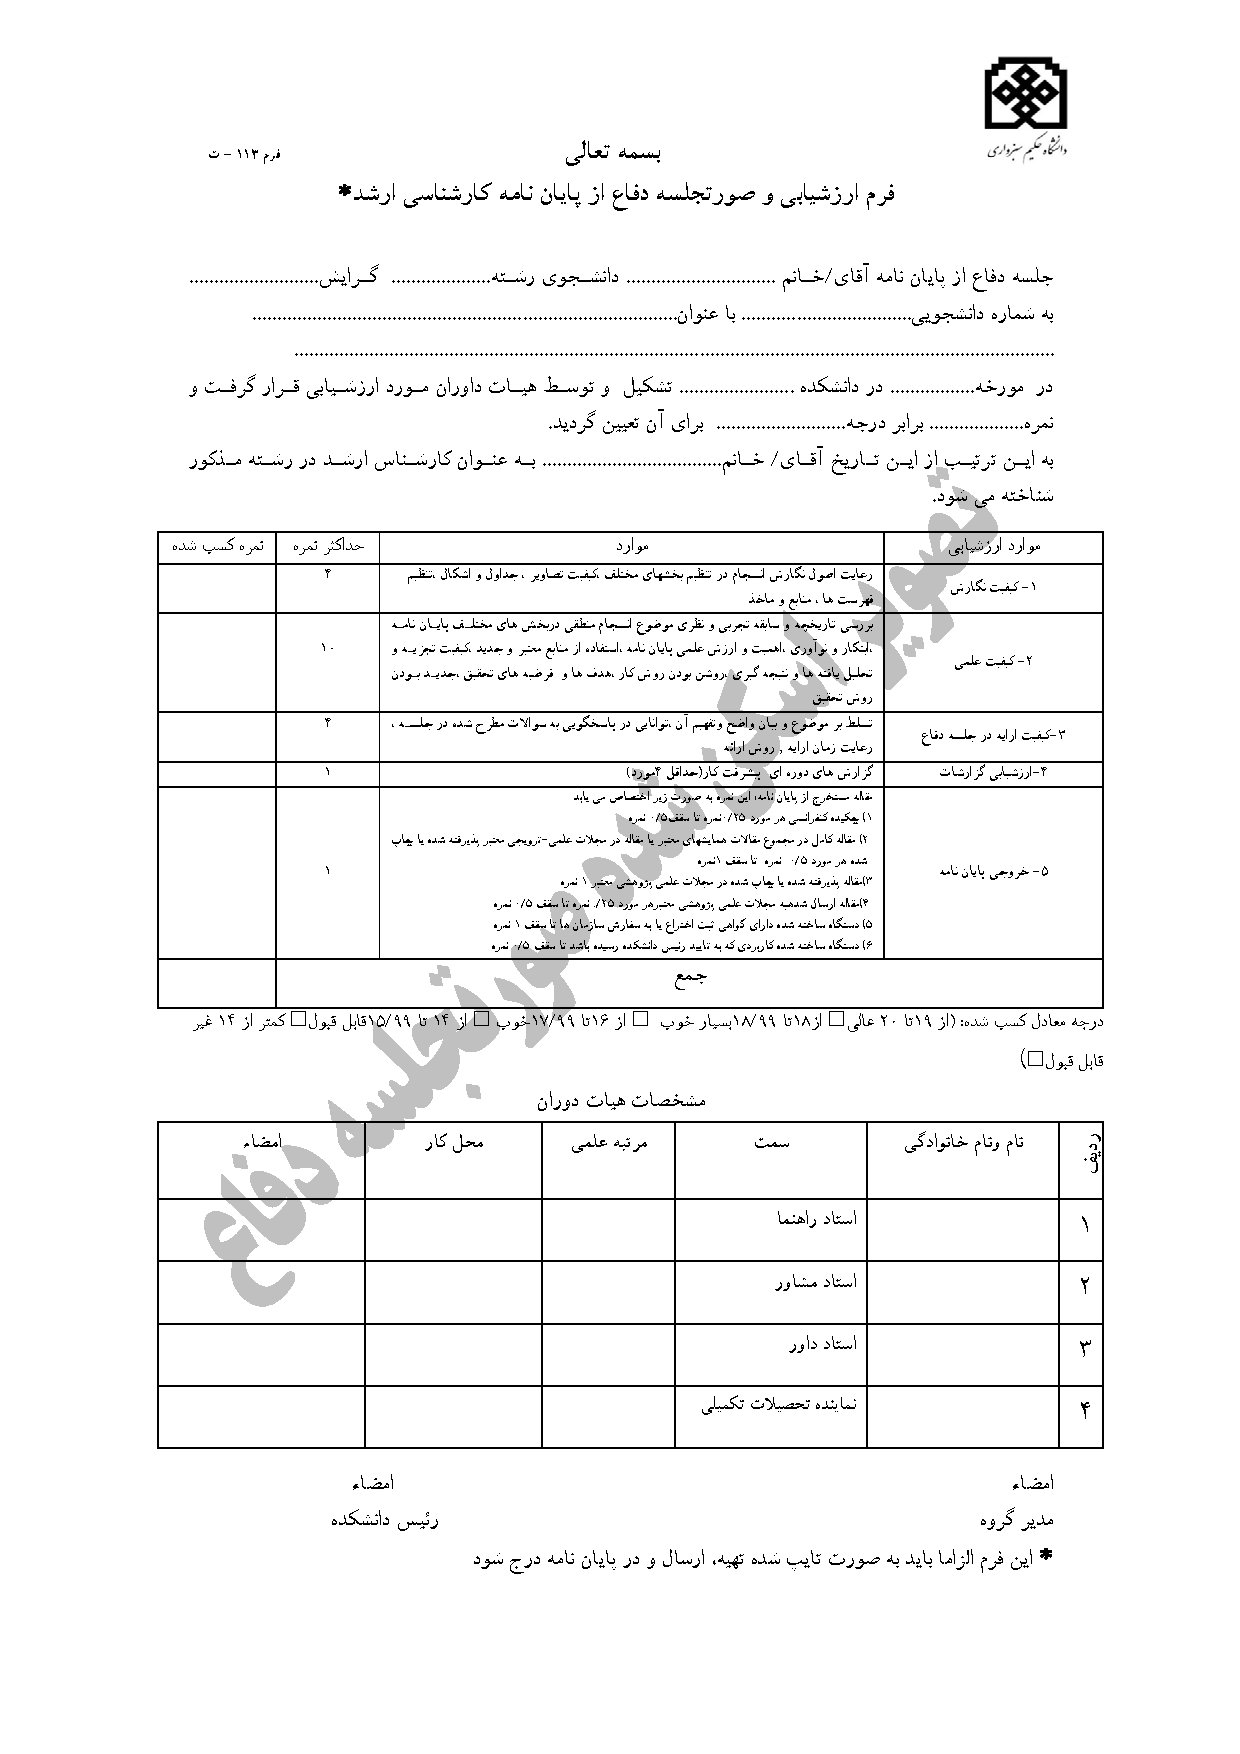
\includepdf{sooratjalaseh.pdf}!
در همان فایل را از حالت توضیح خارج کنید.
\end{enumerate}
دقت داشته باشید که اگر فایل اسکن شده شما، نامی به جز 
\lr{sooratjalaseh}
دارد یا باید نام آنرا به همین عبارت تغییر دهید و یا نام فایل خود را در  دستور فوق قرار دهید.
جدول اطلاعات داوران در فایل
\lr{davaranJadval.tex}
قرار دارد.

\subsection{مراجع}
برای وارد کردن مراجع \پ خود، کافی است فایل 
\lr{MyReferences.bib}
را باز کرده و مراجع خود را مانند مراجع داخل آن، وارد کنید.  سپس از \lr{bibtex} برای تولید مراجع با قالب مناسب استفاده کنید. برای توضیحات بیشتر بخش \ref{Sec:Ref} و پیوست
\eqref{App:App1} را ببینید.


\subsection{واژه‌نامه و نمایه}
برای وارد کردن واژه‌نامه فارسی به انگلیسی و برعکس، چنانچه کاربر مبتدی هستید، بهتر است مانند روش بکار رفته در فایل‌های 
\lr{dicfa2en}
و
\lr{dicen2fa}
عمل کنید. اما چنانچه کاربر پیشرفته هستید، بهتر است از بسته
\lr{glossaries}
استفاده کنید. 
برای وارد کردن نمایه، باید از 
\lr{xindy}
استفاده کنید. 
%زیرا 
%\lr{MakeIndex}
%با حروف «گ»، «چ»، «پ»، «ژ» و «ک» مشکل دارد و ترتیب الفبایی این حروف را رعایت نمی‌کند. همچنین، فاصله بین هر گروه از کلمات در 
%\lr{MakeIndex}،
%به درستی رعایت نمی‌شود که باعث زشت شدن حروف‌چینی این قسمت می‌شود. 
راهنمای چگونگی کار با 
\lr{glossaries} و \lr{xindy} 
را می‌توانید در
 \href{http://wiki.parsilatex.com}{ویکی پارسی‌لاتک} 
 مشاهده فرمایید.

\section{اگر سوالی داشتم، از کی بپرسم؟}
برای پرسیدن سوال های خود موقع حروف‌چینی با زی‌پرشین،  می‌توانید به
 \href{http://qa.parsilatex.com}{سایت پرسش و پاسخ پارسی‌لاتک}%
\LTRfootnote{\url{http://qa.parsilatex.com}}
مراجعه کنید. شما هم می‌توانید روزی به سوال های دیگران در این تالار، جواب بدهید.
بسته ی زی‌پرشین و بسیاری بسته‌های مرتبط با آن مانند \lr{bidi} و \lr{Persian-bib}، مجموعه پارسی‌لاتک، مثالهای مختلف موجود در آن و سایت پارسی‌لاتک همه به صورت داوطلبانه توسط افراد گروه 
\lr{Persian TeX}
و گروه پارسی‌لاتک و بدون هیچ کمک مالی انجام شده‌اند. کار اصلی نوشتن و توسعه زی‌پرشین توسط آقای وفا خلیقی انجام شده است که‌این کار بزرگ را به انجام رساندند.
اگر مایل به کمک به گروه پارسی‌لاتک هستید به سایت گروه پارسی‌لاتک مراجعه فرمایید:
%\begin{center}
 \href{http://www.parsilatex.com}{http://www.parsilatex.com} 
%\end{center}
    
\section{جمع بندی}
در این فصل به بیان مقدمات نحوه استفاده از قالب پایان‌نامه دانشگاه حکیم سبزواری پرداخته شد. گرچه که مطالعه کامل این راهنما مقداری وقت شما را خواهد گرفت، اما مطمئن باشید از اتلاف وقت شما در ادامه کارتان تا حد زیادی جلوگیری خواهد کرد. در نوشتن متن حاضر سعی شده است بیشتر مواردی که عموماً دانشجوان با آن مواجه هستند - و با نگاه ویژه به نیازهای دانشجویان ریاضی - ذکر شود. در ادامه نوشتار نمونه مواردی از درج تصویر، نمودار، کد برنامه، الگوریتم، توضیحات، منابع، فرمول، تعریف، قضیه، مثال و جدول آمده است. توصیه می‌شود یک کپی از کل فایلهای این قالب را جداگانه از نسخه \پ خود نگهداری نمایید تا در صورت نیاز بتوانید مراجعه فرمایید. همچنین توصیه اکید دارم که رفع خطاهایی که احتمالاً با آن مواجه می‌شوید را با آخر موکول نفرمایید و به محض برخورد با خطا، آنرا اشکال‌زدایی نموده و خطا را برطرف فرمایید.

!
و
\verb!% !TEX TS-program = XeLaTeX
% !TeX root=main.tex

\chapter{آشنایی سریع با برخی دستورات لاتک}\label{Chap:chapter2}

در این فصل ویژگی های مهم و پرکاربرد زی‌پرشین و لاتک معرفی می‌شود. برای راهنمایی بیشتر و به کاربردن ویژگی های پیشرفته تر به راهنمای زی‌پرشین و راهنمای لاتک مراجعه کنید. برای آگاهی از دستورات لاتک که‌این خروجی را تولید کرده‌اند فایل \lr{chapter2.tex} را ملاحظه فرمایید.
%\footnote{بیشتر مطالب این بخش از مثال 
%\lr{xepersian\_example.tex}
%گرفته شده‌اند که توسط دوستمان آقای امیرمسعود پورموسی آماده شده بوده است.}

\section{بندها و زیرنویس ها}
هر جایی از نوشتهٔ خود، اگر می خواهید به سر سطر بروید و یک بند تازه را آغاز کنید، باید یک خط را خالی بگذارید.
%\footnote{یعنی دوبار باید کلید \lr{Enter} را بزنید.}
% مانند این:

حالا که یک بند تازه آغاز شده است، یک زیرنویس انگلیسی
\LTRfootnote{English Footnote!}
 هم می نویسیم!
\section{فرمول های ریاضی}\label{formula}

اینجا هم یک فرمول می آوریم که شماره دارد:
\begin{equation}\label{eq:yek}
A=\frac{c}{d}+\frac{q^2}{\sin(\omega t)+\Omega_{12}}
\end{equation}

%\RTLcolumnfootnotes

در لاتک می توان به کمک فرمان 
\lr{\textbackslash label\{\}}
به هر فرمول یک نام نسبت داد. در فرمول بالا نام \lr{eq:yek} را برایش گذاشته‌ایم (پروندهٔ \lr{tex} همراه با این مثال را ببینید). این نام ما را قادر می‌کند که بعداً بتوانیم با فرمان
\lr{\textbackslash ref\{eq:yek\}}
به آن فرمول با شماره ارجاع دهیم. یعنی بنویسیم فرمول \ref{eq:yek}. 
لاتک خودش شمارهٔ این فرمول ها را مدیریت می‌کند. یعنی اگر بعداً فرمولی قبل از این فرمول بنویسیم، خودبه خود شمارهٔ این فرمول و شمارهٔ ارجاع ها به‌این فرمول یکی زیاد می‌شود و لازم نیست نگران شماره گذاری فرمول های خود باشید.

این هم یک فرمول که شماره ندارد:
$$A=|\vec{a}\times \vec{b}| + \sum_{n=0}^\infty C_{ij}$$

این هم عبارتی ریاضی مانند 
$\sqrt{a^2+b^2}$
 که بین متن می آید.

نمایش ارقام در محیط‌های مختلف متفاوت است. به عنوان مثال اگر \lr{0123456789.123} را  در حالت متن و ریاضی فارسی و در حالت معمولی و پررنگ لاتین داشته باشید، خروجی به ترتیب به صورت زیر خواهد بود:
 \begin{LTR}
 \noindent
 0123456789.123\\
 $0123456789.123$\\
 \lr{0123456789.123}\\
\lr{ $\mathbf{0123456789.123}$}\\
\end{LTR}
 ارقام در حالت متن فارسی از قلم فارسی و در متن انگلیسی از قلم انگلیسی گرفته می‌شوند. تغییر نوع و اندازه قلم ارقام در محیط ریاضی با دستور 
\lr{setdigitfont}
در فایل 
\lr{commands}
قابل انجام است. 
   ممکن است خواسته باشید برخی ارقام ریاضی را - مثلاً برای نمایش یک بردار - با حروفی متفاوت نشان دهید، مثل این: 
\begin{LTR}
 \noindent
$\mathsf{0123456789.123}$ 
\end{LTR}


که از دستور 
\verb!\mathsf{0123456789}!
برای نمایش آن استفاده شده است. در این استیل از قلم 
\lr{IRTitr}
در دستور
\verb!\setmathsfdigitfont{IRTitr}!
در فایل 
\lr{commands}
به این منظور استفاده شده است که در صورت نیاز می‌توانید آن‌را تغییر دهید.

\subsection{یک زیربخش}\label{zirbakhsh}

این زیربخش \ref{zirbakhsh} است؛ یعنی یک بخش درون بخش \ref{formula} است.
\subsubsection{یک زیرزیربخش}
این هم یک زیرزیربخش است. در لاتک می‌توانید بخش‌های تودرتو در نوشته تان تعریف کنید تا ساختار منطقی نوشته را به خوبی نشان دهید. می‌توانید به‌این بخش‌ها هم با شماره ارجاع دهید، مثلاً بخش فرمول های ریاضی شماره اش \ref{formula} است.
\section{نوشته‌های فارسی و انگلیسی مخلوط}
نوشتن یک کلمهٔ انگلیسی بین متن فارسی بدیهی است، مانند Example در این جمله.
نوشتن یک عبارت چندکلمه‌ای مانند
 \lr{More than one word} کمی پیچیده تر است.

اگر ناگهان تصمیم بگیرید که یک بند کاملاً انگلیسی را بنویسید، باید:
\begin{latin}
This is an English paragraph from left to right. You can write as much as you want in it.
\end{latin}
\section{افزودن تصویر به نوشته}
پروندهٔ تصویر دلخواه خود را در کنار پروندهٔ \lr{tex} قرار دهید. سپس به روش زیر تصویر را در نوشتهٔ خود بیاورید:
\begin{latin}
\begin{verbatim}
\includegraphics{YourImageFileName}
\end{verbatim}
\end{latin}
به تصویرها هم مانند فرمول ها و بخش‌ها می توان با شماره ارجاع داد. برای جزئیات بیشتر دربارهٔ روش گذاشتن تصویرها در نوشته باید راهنماهای لاتک را بخوانید. نمونه تصاویری در پیوست آمده است که می‌توانید نحوه درج آنها را ملاحظه فرمایید.


\section{محیط های شمارش و نکات}
برای فهرست کردن چندمورد، اگر ترتیب برایمان مهم نباشد:
\begin{itemize}
\item مورد یکم
\item مورد دوم
\item مورد سوم
\end{itemize}
و اگر ترتیب برایمان مهم باشد:
\begin{enumerate}
\item مورد یکم
\item مورد دوم
\item مورد سوم
\end{enumerate}
می توان موردهای تودرتو داشت:
\begin{enumerate}
\item مورد ۱
\item مورد ۲
\begin{enumerate}
\item مورد ۱ از ۲
\item مورد ۲ از ۲
\item مورد ۳ از ۲
\end{enumerate}
\item مورد ۳
\end{enumerate}
شماره گذاری این موردها را هم لاتک انجام می دهد.

\section{تعریف و قضیه}

برای ذکر تعریف، قضیه و مثال مثالهای ذیل را ببینید.

%\textbf{برای ذکر تعریف، قضیه و مثال مثالهای ذیل را ببینید.}
%
%{\iranicfamily برای ذکر تعریف، قضیه و مثال مثالهای ذیل را ببینید.}
%
%\textbf{\emph{ برای ذکر تعریف، قضیه و مثال مثالهای ذیل را ببینید.}}
%
%{\iranicfamily \bf{ برای ذکر تعریف، قضیه و مثال مثالهای ذیل را ببینید.}}

\begin{definition}
مجموعه همه ارزیابی های  (پیوسته)  روی $(X,\tau)$، دامنه توانی احتمالی
\index{دامنه توانی احتمالی}
$ X $
نامیده می‌شود.
\end{definition}
\begin{theorem}[باناخ-آلااغلو]
\index{قضیه باناخ-آلااغلو}
اگر $ V $ یک همسایگی $ 0 $ در فضای برداری 
\index{فضای!برداری}
 توپولوژیکی $ X $ باشد و 
\begin{equation}\label{eq1}
K=\left\lbrace \Lambda \in X^{*}:|\Lambda x|\leqslant 1 ; \ \forall x\in V\right\rbrace,
\end{equation}
آنگاه $ K $،  ضعیف*-فشرده است که در آن، $ X^{*} $ دوگان
\index{فضای!دوگان}
 فضای برداری توپولوژیکی $ X $ است به  طوری که عناصر آن،  تابعی های 
خطی پیوسته
\index{تابعی خطی پیوسته}
 روی $X$ هستند.
\end{theorem}
تساوی \eqref{eq1} یکی از مهم ترین تساوی ها در آنالیز تابعی است که در ادامه، به وفور از آن استفاده می‌شود.
\begin{example}
برای هر فضای مرتب، گردایه 
$$U:=\left\lbrace U\in O: U=\uparrow U\right\rbrace $$
از مجموعه‌های بالایی باز، یک توپولوژی تعریف می‌کند که از توپولوژی اصلی، درشت تر  است.
\end{example}
حال تساوی 
\begin{equation}\label{eq2}
\sum_{n=1}^{+\infty} 3^{n}x+7x=\int_{1}^{n}8nx+\exp{(2nx)}
\end{equation}
را در نظر بگیرید. با مقایسه تساوی \eqref{eq2} با تساوی \eqref{eq1} می توان نتیجه گرفت که ...


\section{چگونگی نوشتن و ارجاع به مراجع}\label{Sec:Ref}

در لاتک به راحتی می توان مراجع خود را نوشت و به آنها ارجاع داد. به عنوان مثال برای معرفی کتاب گنزالس \cite{Gonzalez02book} به عنوان یک مرجع می توان آنرا به صورت زیر معرفی نمود:

\singlespacing
\begin{LTR}
\begin{verbatim}
\bibitem{Gonzalez02book}
Gonzalez, R.C., and Woods, R.E. {\em Digital Image Processing}, 3rd ed..
Prentice-Hall, Inc., Upper Saddle River, NJ, USA, 2006.
\end{verbatim}
\end{LTR}
\doublespacing

در دستورات فوق \lr{Gonzalez02book}  برچسبی است که به‌این مرجع داده شده است و با استفاده از دستور 
\verb!\cite{Gonzalez02book}!
می توان به آن ارجاع داد؛ بدون این که شماره اش را در فهرست مراجع مان بدانیم.

اگر این اولین مرجع ما باشد در قسمت مراجع به صورت زیر خواهد آمد:\\
\begin{latin}

\noindent [1] Gonzalez, Rafael~C. and Woods, Richard~E.  {\em Digital Image Processing}.  Prentice-Hall, 

Inc., Upper Saddle River, NJ, USA, 3rd ed. , 2006.
\end{latin}


این شیوه برای تعداد مراجع کم بد نیست اما اگر فرمت مراجع، ترتیب یا تعداد آنها را خواسته باشید تغییر دهید، به عنوان مثال ابتدا حرف اول نام نویسنده بیاید و سپس نام خانوادگی، باید همه کارها را به صورت دستی انجام دهید.
اگر مایلید کنترل کاملی بر مراجع خود داشته باشید و به راحتی بتوانید قالب مراجع خود را عوض کنید باید از \lr{Bib\TeX} استفاده کنید که درپیوست  \ref{App:App1} به  آن پرداخته خواهد شد.
!
را در فایل 
\lr{main.tex}،
غیرفعال کنید.
برای غیرفعال کردن یک دستور، کافی است در ابتدای آن، یک علامت درصد انگلیسی (\%) بگذارید.
   در غیر این صورت، ابتدا مطالب دو فصل اول  پردازش شده و سپس مطالب فصل ۳ پردازش می‌شود و این کار باعث طولانی شدن زمان اجرا می‌شود. هر زمان که خروجی کل \پ خود را خواستید تمام فصلها را از حالت توضیح خارج کنید.


یک نکته بدیهی که در اینجا وجود دارد، این است که لازم نیست که فصل‌های \پ را به ترتیب تایپ کنید. می‌توانید ابتدا مطالب فصل ۳ را تایپ کنید و سپس مطالب فصل ۱ را تایپ کنید. 
\subsection{فرم ارزشیابی و صورتجلسه دفاع}
فرم ۱۱۳-ت از فرم‌های مربوط به تحصیلات تکمیلی، «فرم ارزشیابی و صورتجلسه دفاع، به همراه مشخصات داوران» است که باید در صفحات آغازین \پ درج شود.
وابسته به اطلاعات \پ این فرم توسط قالب پایان‌نامه آماده می‌شود. اما در نهایت، پس از دفاع باید این فرم اسکن شده و در \پ درج گردد.
برای درج فرم اسکن شده، کافیست:
\begin{enumerate}
\item
دستور 
\verb!\davaranPage!
در اواخر فایل
\lr{faTitle}
را به حالت توضیح درآورید،
\item
  فایل اسکن شده با پسوند 
\lr{PDF}
را در پوشه فایل‌های \پ قرار دهید و
\item
دستور
\verb!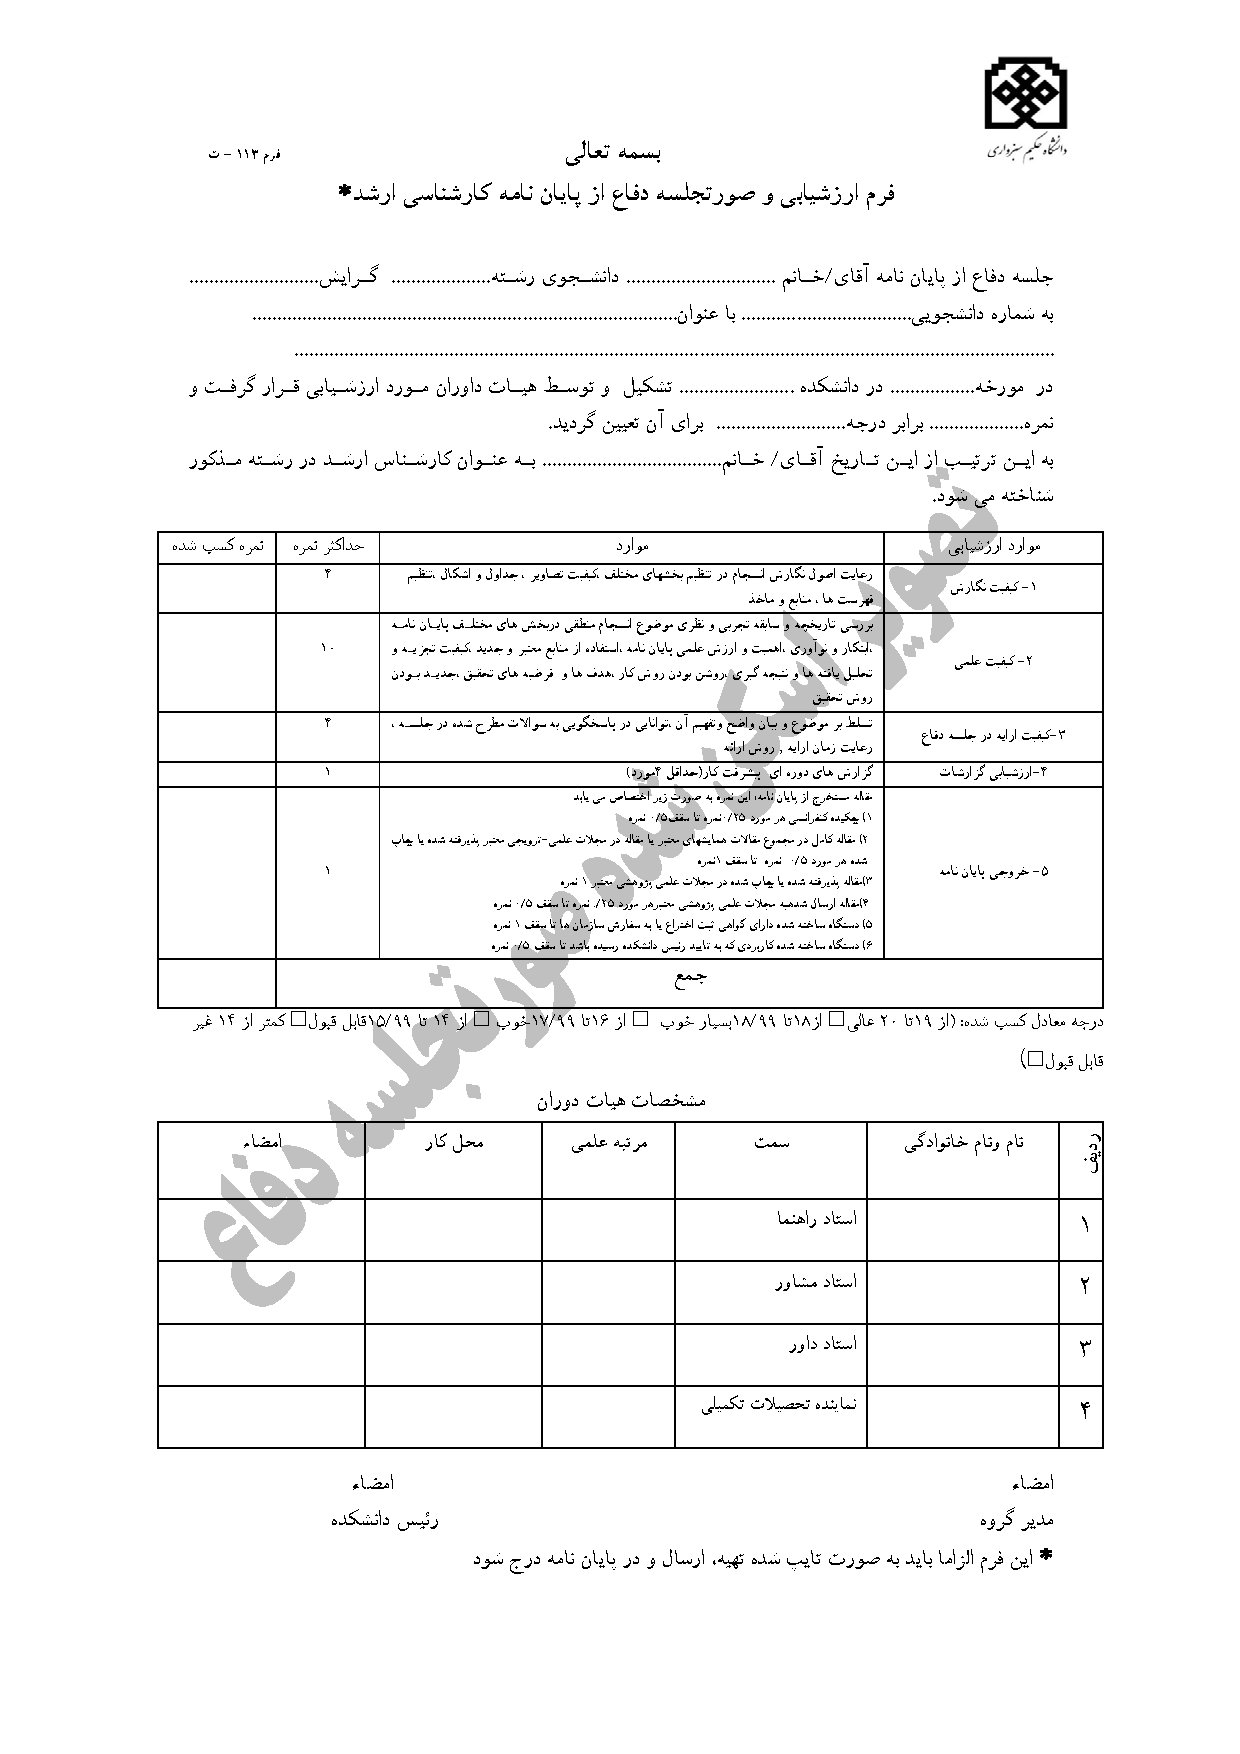
\includepdf{sooratjalaseh.pdf}!
در همان فایل را از حالت توضیح خارج کنید.
\end{enumerate}
دقت داشته باشید که اگر فایل اسکن شده شما، نامی به جز 
\lr{sooratjalaseh}
دارد یا باید نام آنرا به همین عبارت تغییر دهید و یا نام فایل خود را در  دستور فوق قرار دهید.
جدول اطلاعات داوران در فایل
\lr{davaranJadval.tex}
قرار دارد.

\subsection{مراجع}
برای وارد کردن مراجع \پ خود، کافی است فایل 
\lr{MyReferences.bib}
را باز کرده و مراجع خود را مانند مراجع داخل آن، وارد کنید.  سپس از \lr{bibtex} برای تولید مراجع با قالب مناسب استفاده کنید. برای توضیحات بیشتر بخش \ref{Sec:Ref} و پیوست
\eqref{App:App1} را ببینید.


\subsection{واژه‌نامه و نمایه}
برای وارد کردن واژه‌نامه فارسی به انگلیسی و برعکس، چنانچه کاربر مبتدی هستید، بهتر است مانند روش بکار رفته در فایل‌های 
\lr{dicfa2en}
و
\lr{dicen2fa}
عمل کنید. اما چنانچه کاربر پیشرفته هستید، بهتر است از بسته
\lr{glossaries}
استفاده کنید. 
برای وارد کردن نمایه، باید از 
\lr{xindy}
استفاده کنید. 
%زیرا 
%\lr{MakeIndex}
%با حروف «گ»، «چ»، «پ»، «ژ» و «ک» مشکل دارد و ترتیب الفبایی این حروف را رعایت نمی‌کند. همچنین، فاصله بین هر گروه از کلمات در 
%\lr{MakeIndex}،
%به درستی رعایت نمی‌شود که باعث زشت شدن حروف‌چینی این قسمت می‌شود. 
راهنمای چگونگی کار با 
\lr{glossaries} و \lr{xindy} 
را می‌توانید در
 \href{http://wiki.parsilatex.com}{ویکی پارسی‌لاتک} 
 مشاهده فرمایید.

\section{اگر سوالی داشتم، از کی بپرسم؟}
برای پرسیدن سوال های خود موقع حروف‌چینی با زی‌پرشین،  می‌توانید به
 \href{http://qa.parsilatex.com}{سایت پرسش و پاسخ پارسی‌لاتک}%
\LTRfootnote{\url{http://qa.parsilatex.com}}
مراجعه کنید. شما هم می‌توانید روزی به سوال های دیگران در این تالار، جواب بدهید.
بسته ی زی‌پرشین و بسیاری بسته‌های مرتبط با آن مانند \lr{bidi} و \lr{Persian-bib}، مجموعه پارسی‌لاتک، مثالهای مختلف موجود در آن و سایت پارسی‌لاتک همه به صورت داوطلبانه توسط افراد گروه 
\lr{Persian TeX}
و گروه پارسی‌لاتک و بدون هیچ کمک مالی انجام شده‌اند. کار اصلی نوشتن و توسعه زی‌پرشین توسط آقای وفا خلیقی انجام شده است که‌این کار بزرگ را به انجام رساندند.
اگر مایل به کمک به گروه پارسی‌لاتک هستید به سایت گروه پارسی‌لاتک مراجعه فرمایید:
%\begin{center}
 \href{http://www.parsilatex.com}{http://www.parsilatex.com} 
%\end{center}
    
\section{جمع بندی}
در این فصل به بیان مقدمات نحوه استفاده از قالب پایان‌نامه دانشگاه حکیم سبزواری پرداخته شد. گرچه که مطالعه کامل این راهنما مقداری وقت شما را خواهد گرفت، اما مطمئن باشید از اتلاف وقت شما در ادامه کارتان تا حد زیادی جلوگیری خواهد کرد. در نوشتن متن حاضر سعی شده است بیشتر مواردی که عموماً دانشجوان با آن مواجه هستند - و با نگاه ویژه به نیازهای دانشجویان ریاضی - ذکر شود. در ادامه نوشتار نمونه مواردی از درج تصویر، نمودار، کد برنامه، الگوریتم، توضیحات، منابع، فرمول، تعریف، قضیه، مثال و جدول آمده است. توصیه می‌شود یک کپی از کل فایلهای این قالب را جداگانه از نسخه \پ خود نگهداری نمایید تا در صورت نیاز بتوانید مراجعه فرمایید. همچنین توصیه اکید دارم که رفع خطاهایی که احتمالاً با آن مواجه می‌شوید را با آخر موکول نفرمایید و به محض برخورد با خطا، آنرا اشکال‌زدایی نموده و خطا را برطرف فرمایید.

!
و
\verb!% !TEX TS-program = XeLaTeX
% !TeX root=main.tex

\chapter{آشنایی سریع با برخی دستورات لاتک}\label{Chap:chapter2}

در این فصل ویژگی های مهم و پرکاربرد زی‌پرشین و لاتک معرفی می‌شود. برای راهنمایی بیشتر و به کاربردن ویژگی های پیشرفته تر به راهنمای زی‌پرشین و راهنمای لاتک مراجعه کنید. برای آگاهی از دستورات لاتک که‌این خروجی را تولید کرده‌اند فایل \lr{chapter2.tex} را ملاحظه فرمایید.
%\footnote{بیشتر مطالب این بخش از مثال 
%\lr{xepersian\_example.tex}
%گرفته شده‌اند که توسط دوستمان آقای امیرمسعود پورموسی آماده شده بوده است.}

\section{بندها و زیرنویس ها}
هر جایی از نوشتهٔ خود، اگر می خواهید به سر سطر بروید و یک بند تازه را آغاز کنید، باید یک خط را خالی بگذارید.
%\footnote{یعنی دوبار باید کلید \lr{Enter} را بزنید.}
% مانند این:

حالا که یک بند تازه آغاز شده است، یک زیرنویس انگلیسی
\LTRfootnote{English Footnote!}
 هم می نویسیم!
\section{فرمول های ریاضی}\label{formula}

اینجا هم یک فرمول می آوریم که شماره دارد:
\begin{equation}\label{eq:yek}
A=\frac{c}{d}+\frac{q^2}{\sin(\omega t)+\Omega_{12}}
\end{equation}

%\RTLcolumnfootnotes

در لاتک می توان به کمک فرمان 
\lr{\textbackslash label\{\}}
به هر فرمول یک نام نسبت داد. در فرمول بالا نام \lr{eq:yek} را برایش گذاشته‌ایم (پروندهٔ \lr{tex} همراه با این مثال را ببینید). این نام ما را قادر می‌کند که بعداً بتوانیم با فرمان
\lr{\textbackslash ref\{eq:yek\}}
به آن فرمول با شماره ارجاع دهیم. یعنی بنویسیم فرمول \ref{eq:yek}. 
لاتک خودش شمارهٔ این فرمول ها را مدیریت می‌کند. یعنی اگر بعداً فرمولی قبل از این فرمول بنویسیم، خودبه خود شمارهٔ این فرمول و شمارهٔ ارجاع ها به‌این فرمول یکی زیاد می‌شود و لازم نیست نگران شماره گذاری فرمول های خود باشید.

این هم یک فرمول که شماره ندارد:
$$A=|\vec{a}\times \vec{b}| + \sum_{n=0}^\infty C_{ij}$$

این هم عبارتی ریاضی مانند 
$\sqrt{a^2+b^2}$
 که بین متن می آید.

نمایش ارقام در محیط‌های مختلف متفاوت است. به عنوان مثال اگر \lr{0123456789.123} را  در حالت متن و ریاضی فارسی و در حالت معمولی و پررنگ لاتین داشته باشید، خروجی به ترتیب به صورت زیر خواهد بود:
 \begin{LTR}
 \noindent
 0123456789.123\\
 $0123456789.123$\\
 \lr{0123456789.123}\\
\lr{ $\mathbf{0123456789.123}$}\\
\end{LTR}
 ارقام در حالت متن فارسی از قلم فارسی و در متن انگلیسی از قلم انگلیسی گرفته می‌شوند. تغییر نوع و اندازه قلم ارقام در محیط ریاضی با دستور 
\lr{setdigitfont}
در فایل 
\lr{commands}
قابل انجام است. 
   ممکن است خواسته باشید برخی ارقام ریاضی را - مثلاً برای نمایش یک بردار - با حروفی متفاوت نشان دهید، مثل این: 
\begin{LTR}
 \noindent
$\mathsf{0123456789.123}$ 
\end{LTR}


که از دستور 
\verb!\mathsf{0123456789}!
برای نمایش آن استفاده شده است. در این استیل از قلم 
\lr{IRTitr}
در دستور
\verb!\setmathsfdigitfont{IRTitr}!
در فایل 
\lr{commands}
به این منظور استفاده شده است که در صورت نیاز می‌توانید آن‌را تغییر دهید.

\subsection{یک زیربخش}\label{zirbakhsh}

این زیربخش \ref{zirbakhsh} است؛ یعنی یک بخش درون بخش \ref{formula} است.
\subsubsection{یک زیرزیربخش}
این هم یک زیرزیربخش است. در لاتک می‌توانید بخش‌های تودرتو در نوشته تان تعریف کنید تا ساختار منطقی نوشته را به خوبی نشان دهید. می‌توانید به‌این بخش‌ها هم با شماره ارجاع دهید، مثلاً بخش فرمول های ریاضی شماره اش \ref{formula} است.
\section{نوشته‌های فارسی و انگلیسی مخلوط}
نوشتن یک کلمهٔ انگلیسی بین متن فارسی بدیهی است، مانند Example در این جمله.
نوشتن یک عبارت چندکلمه‌ای مانند
 \lr{More than one word} کمی پیچیده تر است.

اگر ناگهان تصمیم بگیرید که یک بند کاملاً انگلیسی را بنویسید، باید:
\begin{latin}
This is an English paragraph from left to right. You can write as much as you want in it.
\end{latin}
\section{افزودن تصویر به نوشته}
پروندهٔ تصویر دلخواه خود را در کنار پروندهٔ \lr{tex} قرار دهید. سپس به روش زیر تصویر را در نوشتهٔ خود بیاورید:
\begin{latin}
\begin{verbatim}
\includegraphics{YourImageFileName}
\end{verbatim}
\end{latin}
به تصویرها هم مانند فرمول ها و بخش‌ها می توان با شماره ارجاع داد. برای جزئیات بیشتر دربارهٔ روش گذاشتن تصویرها در نوشته باید راهنماهای لاتک را بخوانید. نمونه تصاویری در پیوست آمده است که می‌توانید نحوه درج آنها را ملاحظه فرمایید.


\section{محیط های شمارش و نکات}
برای فهرست کردن چندمورد، اگر ترتیب برایمان مهم نباشد:
\begin{itemize}
\item مورد یکم
\item مورد دوم
\item مورد سوم
\end{itemize}
و اگر ترتیب برایمان مهم باشد:
\begin{enumerate}
\item مورد یکم
\item مورد دوم
\item مورد سوم
\end{enumerate}
می توان موردهای تودرتو داشت:
\begin{enumerate}
\item مورد ۱
\item مورد ۲
\begin{enumerate}
\item مورد ۱ از ۲
\item مورد ۲ از ۲
\item مورد ۳ از ۲
\end{enumerate}
\item مورد ۳
\end{enumerate}
شماره گذاری این موردها را هم لاتک انجام می دهد.

\section{تعریف و قضیه}

برای ذکر تعریف، قضیه و مثال مثالهای ذیل را ببینید.

%\textbf{برای ذکر تعریف، قضیه و مثال مثالهای ذیل را ببینید.}
%
%{\iranicfamily برای ذکر تعریف، قضیه و مثال مثالهای ذیل را ببینید.}
%
%\textbf{\emph{ برای ذکر تعریف، قضیه و مثال مثالهای ذیل را ببینید.}}
%
%{\iranicfamily \bf{ برای ذکر تعریف، قضیه و مثال مثالهای ذیل را ببینید.}}

\begin{definition}
مجموعه همه ارزیابی های  (پیوسته)  روی $(X,\tau)$، دامنه توانی احتمالی
\index{دامنه توانی احتمالی}
$ X $
نامیده می‌شود.
\end{definition}
\begin{theorem}[باناخ-آلااغلو]
\index{قضیه باناخ-آلااغلو}
اگر $ V $ یک همسایگی $ 0 $ در فضای برداری 
\index{فضای!برداری}
 توپولوژیکی $ X $ باشد و 
\begin{equation}\label{eq1}
K=\left\lbrace \Lambda \in X^{*}:|\Lambda x|\leqslant 1 ; \ \forall x\in V\right\rbrace,
\end{equation}
آنگاه $ K $،  ضعیف*-فشرده است که در آن، $ X^{*} $ دوگان
\index{فضای!دوگان}
 فضای برداری توپولوژیکی $ X $ است به  طوری که عناصر آن،  تابعی های 
خطی پیوسته
\index{تابعی خطی پیوسته}
 روی $X$ هستند.
\end{theorem}
تساوی \eqref{eq1} یکی از مهم ترین تساوی ها در آنالیز تابعی است که در ادامه، به وفور از آن استفاده می‌شود.
\begin{example}
برای هر فضای مرتب، گردایه 
$$U:=\left\lbrace U\in O: U=\uparrow U\right\rbrace $$
از مجموعه‌های بالایی باز، یک توپولوژی تعریف می‌کند که از توپولوژی اصلی، درشت تر  است.
\end{example}
حال تساوی 
\begin{equation}\label{eq2}
\sum_{n=1}^{+\infty} 3^{n}x+7x=\int_{1}^{n}8nx+\exp{(2nx)}
\end{equation}
را در نظر بگیرید. با مقایسه تساوی \eqref{eq2} با تساوی \eqref{eq1} می توان نتیجه گرفت که ...


\section{چگونگی نوشتن و ارجاع به مراجع}\label{Sec:Ref}

در لاتک به راحتی می توان مراجع خود را نوشت و به آنها ارجاع داد. به عنوان مثال برای معرفی کتاب گنزالس \cite{Gonzalez02book} به عنوان یک مرجع می توان آنرا به صورت زیر معرفی نمود:

\singlespacing
\begin{LTR}
\begin{verbatim}
\bibitem{Gonzalez02book}
Gonzalez, R.C., and Woods, R.E. {\em Digital Image Processing}, 3rd ed..
Prentice-Hall, Inc., Upper Saddle River, NJ, USA, 2006.
\end{verbatim}
\end{LTR}
\doublespacing

در دستورات فوق \lr{Gonzalez02book}  برچسبی است که به‌این مرجع داده شده است و با استفاده از دستور 
\verb!\cite{Gonzalez02book}!
می توان به آن ارجاع داد؛ بدون این که شماره اش را در فهرست مراجع مان بدانیم.

اگر این اولین مرجع ما باشد در قسمت مراجع به صورت زیر خواهد آمد:\\
\begin{latin}

\noindent [1] Gonzalez, Rafael~C. and Woods, Richard~E.  {\em Digital Image Processing}.  Prentice-Hall, 

Inc., Upper Saddle River, NJ, USA, 3rd ed. , 2006.
\end{latin}


این شیوه برای تعداد مراجع کم بد نیست اما اگر فرمت مراجع، ترتیب یا تعداد آنها را خواسته باشید تغییر دهید، به عنوان مثال ابتدا حرف اول نام نویسنده بیاید و سپس نام خانوادگی، باید همه کارها را به صورت دستی انجام دهید.
اگر مایلید کنترل کاملی بر مراجع خود داشته باشید و به راحتی بتوانید قالب مراجع خود را عوض کنید باید از \lr{Bib\TeX} استفاده کنید که درپیوست  \ref{App:App1} به  آن پرداخته خواهد شد.
!
را در فایل 
\lr{main.tex}،
غیرفعال کنید.
برای غیرفعال کردن یک دستور، کافی است در ابتدای آن، یک علامت درصد انگلیسی (\%) بگذارید.
   در غیر این صورت، ابتدا مطالب دو فصل اول  پردازش شده و سپس مطالب فصل ۳ پردازش می‌شود و این کار باعث طولانی شدن زمان اجرا می‌شود. هر زمان که خروجی کل \پ خود را خواستید تمام فصلها را از حالت توضیح خارج کنید.


یک نکته بدیهی که در اینجا وجود دارد، این است که لازم نیست که فصل‌های \پ را به ترتیب تایپ کنید. می‌توانید ابتدا مطالب فصل ۳ را تایپ کنید و سپس مطالب فصل ۱ را تایپ کنید. 
\subsection{فرم ارزشیابی و صورتجلسه دفاع}
فرم ۱۱۳-ت از فرم‌های مربوط به تحصیلات تکمیلی، «فرم ارزشیابی و صورتجلسه دفاع، به همراه مشخصات داوران» است که باید در صفحات آغازین \پ درج شود.
وابسته به اطلاعات \پ این فرم توسط قالب پایان‌نامه آماده می‌شود. اما در نهایت، پس از دفاع باید این فرم اسکن شده و در \پ درج گردد.
برای درج فرم اسکن شده، کافیست:
\begin{enumerate}
\item
دستور 
\verb!\davaranPage!
در اواخر فایل
\lr{faTitle}
را به حالت توضیح درآورید،
\item
  فایل اسکن شده با پسوند 
\lr{PDF}
را در پوشه فایل‌های \پ قرار دهید و
\item
دستور
\verb!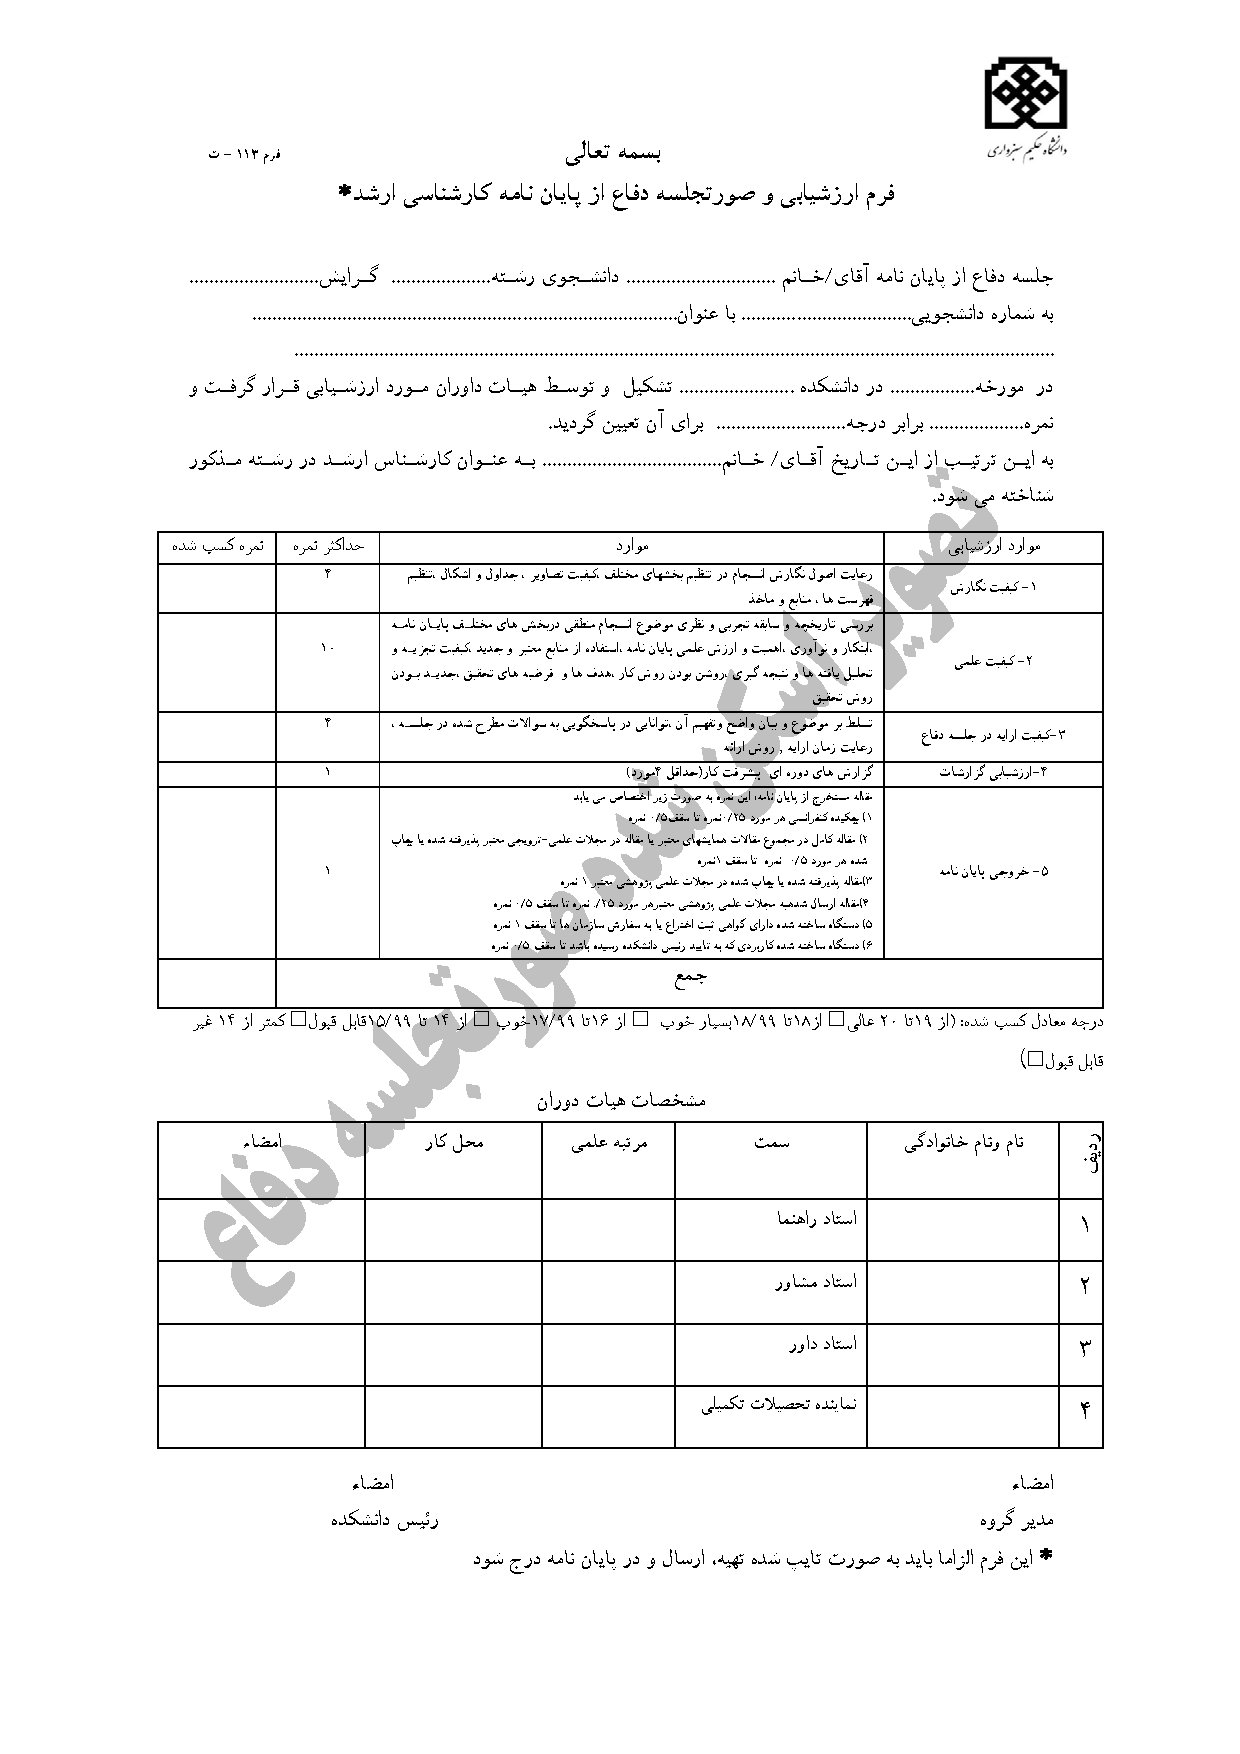
\includepdf{sooratjalaseh.pdf}!
در همان فایل را از حالت توضیح خارج کنید.
\end{enumerate}
دقت داشته باشید که اگر فایل اسکن شده شما، نامی به جز 
\lr{sooratjalaseh}
دارد یا باید نام آنرا به همین عبارت تغییر دهید و یا نام فایل خود را در  دستور فوق قرار دهید.
جدول اطلاعات داوران در فایل
\lr{davaranJadval.tex}
قرار دارد.

\subsection{مراجع}
برای وارد کردن مراجع \پ خود، کافی است فایل 
\lr{MyReferences.bib}
را باز کرده و مراجع خود را مانند مراجع داخل آن، وارد کنید.  سپس از \lr{bibtex} برای تولید مراجع با قالب مناسب استفاده کنید. برای توضیحات بیشتر بخش \ref{Sec:Ref} و پیوست
\eqref{App:App1} را ببینید.


\subsection{واژه‌نامه و نمایه}
برای وارد کردن واژه‌نامه فارسی به انگلیسی و برعکس، چنانچه کاربر مبتدی هستید، بهتر است مانند روش بکار رفته در فایل‌های 
\lr{dicfa2en}
و
\lr{dicen2fa}
عمل کنید. اما چنانچه کاربر پیشرفته هستید، بهتر است از بسته
\lr{glossaries}
استفاده کنید. 
برای وارد کردن نمایه، باید از 
\lr{xindy}
استفاده کنید. 
%زیرا 
%\lr{MakeIndex}
%با حروف «گ»، «چ»، «پ»، «ژ» و «ک» مشکل دارد و ترتیب الفبایی این حروف را رعایت نمی‌کند. همچنین، فاصله بین هر گروه از کلمات در 
%\lr{MakeIndex}،
%به درستی رعایت نمی‌شود که باعث زشت شدن حروف‌چینی این قسمت می‌شود. 
راهنمای چگونگی کار با 
\lr{glossaries} و \lr{xindy} 
را می‌توانید در
 \href{http://wiki.parsilatex.com}{ویکی پارسی‌لاتک} 
 مشاهده فرمایید.

\section{اگر سوالی داشتم، از کی بپرسم؟}
برای پرسیدن سوال های خود موقع حروف‌چینی با زی‌پرشین،  می‌توانید به
 \href{http://qa.parsilatex.com}{سایت پرسش و پاسخ پارسی‌لاتک}%
\LTRfootnote{\url{http://qa.parsilatex.com}}
مراجعه کنید. شما هم می‌توانید روزی به سوال های دیگران در این تالار، جواب بدهید.
بسته ی زی‌پرشین و بسیاری بسته‌های مرتبط با آن مانند \lr{bidi} و \lr{Persian-bib}، مجموعه پارسی‌لاتک، مثالهای مختلف موجود در آن و سایت پارسی‌لاتک همه به صورت داوطلبانه توسط افراد گروه 
\lr{Persian TeX}
و گروه پارسی‌لاتک و بدون هیچ کمک مالی انجام شده‌اند. کار اصلی نوشتن و توسعه زی‌پرشین توسط آقای وفا خلیقی انجام شده است که‌این کار بزرگ را به انجام رساندند.
اگر مایل به کمک به گروه پارسی‌لاتک هستید به سایت گروه پارسی‌لاتک مراجعه فرمایید:
%\begin{center}
 \href{http://www.parsilatex.com}{http://www.parsilatex.com} 
%\end{center}
    
\section{جمع بندی}
در این فصل به بیان مقدمات نحوه استفاده از قالب پایان‌نامه دانشگاه حکیم سبزواری پرداخته شد. گرچه که مطالعه کامل این راهنما مقداری وقت شما را خواهد گرفت، اما مطمئن باشید از اتلاف وقت شما در ادامه کارتان تا حد زیادی جلوگیری خواهد کرد. در نوشتن متن حاضر سعی شده است بیشتر مواردی که عموماً دانشجوان با آن مواجه هستند - و با نگاه ویژه به نیازهای دانشجویان ریاضی - ذکر شود. در ادامه نوشتار نمونه مواردی از درج تصویر، نمودار، کد برنامه، الگوریتم، توضیحات، منابع، فرمول، تعریف، قضیه، مثال و جدول آمده است. توصیه می‌شود یک کپی از کل فایلهای این قالب را جداگانه از نسخه \پ خود نگهداری نمایید تا در صورت نیاز بتوانید مراجعه فرمایید. همچنین توصیه اکید دارم که رفع خطاهایی که احتمالاً با آن مواجه می‌شوید را با آخر موکول نفرمایید و به محض برخورد با خطا، آنرا اشکال‌زدایی نموده و خطا را برطرف فرمایید.

		% فصل اول: مقدمه
% !TEX TS-program = XeLaTeX
% !TeX root=main.tex

\chapter{آشنایی سریع با برخی دستورات لاتک}\label{Chap:chapter2}

در این فصل ویژگی های مهم و پرکاربرد زی‌پرشین و لاتک معرفی می‌شود. برای راهنمایی بیشتر و به کاربردن ویژگی های پیشرفته تر به راهنمای زی‌پرشین و راهنمای لاتک مراجعه کنید. برای آگاهی از دستورات لاتک که‌این خروجی را تولید کرده‌اند فایل \lr{chapter2.tex} را ملاحظه فرمایید.
%\footnote{بیشتر مطالب این بخش از مثال 
%\lr{xepersian\_example.tex}
%گرفته شده‌اند که توسط دوستمان آقای امیرمسعود پورموسی آماده شده بوده است.}

\section{بندها و زیرنویس ها}
هر جایی از نوشتهٔ خود، اگر می خواهید به سر سطر بروید و یک بند تازه را آغاز کنید، باید یک خط را خالی بگذارید.
%\footnote{یعنی دوبار باید کلید \lr{Enter} را بزنید.}
% مانند این:

حالا که یک بند تازه آغاز شده است، یک زیرنویس انگلیسی
\LTRfootnote{English Footnote!}
 هم می نویسیم!
\section{فرمول های ریاضی}\label{formula}

اینجا هم یک فرمول می آوریم که شماره دارد:
\begin{equation}\label{eq:yek}
A=\frac{c}{d}+\frac{q^2}{\sin(\omega t)+\Omega_{12}}
\end{equation}

%\RTLcolumnfootnotes

در لاتک می توان به کمک فرمان 
\lr{\textbackslash label\{\}}
به هر فرمول یک نام نسبت داد. در فرمول بالا نام \lr{eq:yek} را برایش گذاشته‌ایم (پروندهٔ \lr{tex} همراه با این مثال را ببینید). این نام ما را قادر می‌کند که بعداً بتوانیم با فرمان
\lr{\textbackslash ref\{eq:yek\}}
به آن فرمول با شماره ارجاع دهیم. یعنی بنویسیم فرمول \ref{eq:yek}. 
لاتک خودش شمارهٔ این فرمول ها را مدیریت می‌کند. یعنی اگر بعداً فرمولی قبل از این فرمول بنویسیم، خودبه خود شمارهٔ این فرمول و شمارهٔ ارجاع ها به‌این فرمول یکی زیاد می‌شود و لازم نیست نگران شماره گذاری فرمول های خود باشید.

این هم یک فرمول که شماره ندارد:
$$A=|\vec{a}\times \vec{b}| + \sum_{n=0}^\infty C_{ij}$$

این هم عبارتی ریاضی مانند 
$\sqrt{a^2+b^2}$
 که بین متن می آید.

نمایش ارقام در محیط‌های مختلف متفاوت است. به عنوان مثال اگر \lr{0123456789.123} را  در حالت متن و ریاضی فارسی و در حالت معمولی و پررنگ لاتین داشته باشید، خروجی به ترتیب به صورت زیر خواهد بود:
 \begin{LTR}
 \noindent
 0123456789.123\\
 $0123456789.123$\\
 \lr{0123456789.123}\\
\lr{ $\mathbf{0123456789.123}$}\\
\end{LTR}
 ارقام در حالت متن فارسی از قلم فارسی و در متن انگلیسی از قلم انگلیسی گرفته می‌شوند. تغییر نوع و اندازه قلم ارقام در محیط ریاضی با دستور 
\lr{setdigitfont}
در فایل 
\lr{commands}
قابل انجام است. 
   ممکن است خواسته باشید برخی ارقام ریاضی را - مثلاً برای نمایش یک بردار - با حروفی متفاوت نشان دهید، مثل این: 
\begin{LTR}
 \noindent
$\mathsf{0123456789.123}$ 
\end{LTR}


که از دستور 
\verb!\mathsf{0123456789}!
برای نمایش آن استفاده شده است. در این استیل از قلم 
\lr{IRTitr}
در دستور
\verb!\setmathsfdigitfont{IRTitr}!
در فایل 
\lr{commands}
به این منظور استفاده شده است که در صورت نیاز می‌توانید آن‌را تغییر دهید.

\subsection{یک زیربخش}\label{zirbakhsh}

این زیربخش \ref{zirbakhsh} است؛ یعنی یک بخش درون بخش \ref{formula} است.
\subsubsection{یک زیرزیربخش}
این هم یک زیرزیربخش است. در لاتک می‌توانید بخش‌های تودرتو در نوشته تان تعریف کنید تا ساختار منطقی نوشته را به خوبی نشان دهید. می‌توانید به‌این بخش‌ها هم با شماره ارجاع دهید، مثلاً بخش فرمول های ریاضی شماره اش \ref{formula} است.
\section{نوشته‌های فارسی و انگلیسی مخلوط}
نوشتن یک کلمهٔ انگلیسی بین متن فارسی بدیهی است، مانند Example در این جمله.
نوشتن یک عبارت چندکلمه‌ای مانند
 \lr{More than one word} کمی پیچیده تر است.

اگر ناگهان تصمیم بگیرید که یک بند کاملاً انگلیسی را بنویسید، باید:
\begin{latin}
This is an English paragraph from left to right. You can write as much as you want in it.
\end{latin}
\section{افزودن تصویر به نوشته}
پروندهٔ تصویر دلخواه خود را در کنار پروندهٔ \lr{tex} قرار دهید. سپس به روش زیر تصویر را در نوشتهٔ خود بیاورید:
\begin{latin}
\begin{verbatim}
\includegraphics{YourImageFileName}
\end{verbatim}
\end{latin}
به تصویرها هم مانند فرمول ها و بخش‌ها می توان با شماره ارجاع داد. برای جزئیات بیشتر دربارهٔ روش گذاشتن تصویرها در نوشته باید راهنماهای لاتک را بخوانید. نمونه تصاویری در پیوست آمده است که می‌توانید نحوه درج آنها را ملاحظه فرمایید.


\section{محیط های شمارش و نکات}
برای فهرست کردن چندمورد، اگر ترتیب برایمان مهم نباشد:
\begin{itemize}
\item مورد یکم
\item مورد دوم
\item مورد سوم
\end{itemize}
و اگر ترتیب برایمان مهم باشد:
\begin{enumerate}
\item مورد یکم
\item مورد دوم
\item مورد سوم
\end{enumerate}
می توان موردهای تودرتو داشت:
\begin{enumerate}
\item مورد ۱
\item مورد ۲
\begin{enumerate}
\item مورد ۱ از ۲
\item مورد ۲ از ۲
\item مورد ۳ از ۲
\end{enumerate}
\item مورد ۳
\end{enumerate}
شماره گذاری این موردها را هم لاتک انجام می دهد.

\section{تعریف و قضیه}

برای ذکر تعریف، قضیه و مثال مثالهای ذیل را ببینید.

%\textbf{برای ذکر تعریف، قضیه و مثال مثالهای ذیل را ببینید.}
%
%{\iranicfamily برای ذکر تعریف، قضیه و مثال مثالهای ذیل را ببینید.}
%
%\textbf{\emph{ برای ذکر تعریف، قضیه و مثال مثالهای ذیل را ببینید.}}
%
%{\iranicfamily \bf{ برای ذکر تعریف، قضیه و مثال مثالهای ذیل را ببینید.}}

\begin{definition}
مجموعه همه ارزیابی های  (پیوسته)  روی $(X,\tau)$، دامنه توانی احتمالی
\index{دامنه توانی احتمالی}
$ X $
نامیده می‌شود.
\end{definition}
\begin{theorem}[باناخ-آلااغلو]
\index{قضیه باناخ-آلااغلو}
اگر $ V $ یک همسایگی $ 0 $ در فضای برداری 
\index{فضای!برداری}
 توپولوژیکی $ X $ باشد و 
\begin{equation}\label{eq1}
K=\left\lbrace \Lambda \in X^{*}:|\Lambda x|\leqslant 1 ; \ \forall x\in V\right\rbrace,
\end{equation}
آنگاه $ K $،  ضعیف*-فشرده است که در آن، $ X^{*} $ دوگان
\index{فضای!دوگان}
 فضای برداری توپولوژیکی $ X $ است به  طوری که عناصر آن،  تابعی های 
خطی پیوسته
\index{تابعی خطی پیوسته}
 روی $X$ هستند.
\end{theorem}
تساوی \eqref{eq1} یکی از مهم ترین تساوی ها در آنالیز تابعی است که در ادامه، به وفور از آن استفاده می‌شود.
\begin{example}
برای هر فضای مرتب، گردایه 
$$U:=\left\lbrace U\in O: U=\uparrow U\right\rbrace $$
از مجموعه‌های بالایی باز، یک توپولوژی تعریف می‌کند که از توپولوژی اصلی، درشت تر  است.
\end{example}
حال تساوی 
\begin{equation}\label{eq2}
\sum_{n=1}^{+\infty} 3^{n}x+7x=\int_{1}^{n}8nx+\exp{(2nx)}
\end{equation}
را در نظر بگیرید. با مقایسه تساوی \eqref{eq2} با تساوی \eqref{eq1} می توان نتیجه گرفت که ...


\section{چگونگی نوشتن و ارجاع به مراجع}\label{Sec:Ref}

در لاتک به راحتی می توان مراجع خود را نوشت و به آنها ارجاع داد. به عنوان مثال برای معرفی کتاب گنزالس \cite{Gonzalez02book} به عنوان یک مرجع می توان آنرا به صورت زیر معرفی نمود:

\singlespacing
\begin{LTR}
\begin{verbatim}
\bibitem{Gonzalez02book}
Gonzalez, R.C., and Woods, R.E. {\em Digital Image Processing}, 3rd ed..
Prentice-Hall, Inc., Upper Saddle River, NJ, USA, 2006.
\end{verbatim}
\end{LTR}
\doublespacing

در دستورات فوق \lr{Gonzalez02book}  برچسبی است که به‌این مرجع داده شده است و با استفاده از دستور 
\verb!\cite{Gonzalez02book}!
می توان به آن ارجاع داد؛ بدون این که شماره اش را در فهرست مراجع مان بدانیم.

اگر این اولین مرجع ما باشد در قسمت مراجع به صورت زیر خواهد آمد:\\
\begin{latin}

\noindent [1] Gonzalez, Rafael~C. and Woods, Richard~E.  {\em Digital Image Processing}.  Prentice-Hall, 

Inc., Upper Saddle River, NJ, USA, 3rd ed. , 2006.
\end{latin}


این شیوه برای تعداد مراجع کم بد نیست اما اگر فرمت مراجع، ترتیب یا تعداد آنها را خواسته باشید تغییر دهید، به عنوان مثال ابتدا حرف اول نام نویسنده بیاید و سپس نام خانوادگی، باید همه کارها را به صورت دستی انجام دهید.
اگر مایلید کنترل کاملی بر مراجع خود داشته باشید و به راحتی بتوانید قالب مراجع خود را عوض کنید باید از \lr{Bib\TeX} استفاده کنید که درپیوست  \ref{App:App1} به  آن پرداخته خواهد شد.
		% فصل دوم: آشنایی مقدماتی با لاتک

% مراجع
{
\onehalfspacing
\bibliographystyle{unsrt-fa}
\bibliography{MyReferences}
}

% عدم نمایش بخشها و زیربخشهای پیوستها در فهرست مطالب
\addtocontents{toc}{\protect\setcounter{tocdepth}{0}}
\appendix                           %فصلهای پس از این قسمت به عنوان ضمیمه خواهند آمد.
% پیوست اول: مدیریت مراجع در لاتک، درج نمودار، تصویر، جدول و ...
% !TEX TS-program = XeLaTeX
% !TeX root=main.tex
% دستورات زیر باید در اولین فایل پیوست باشند. آنها را حذف نکنید! در غیراینصورت در فهرست مطالب به جای عبارت پیوست عبارت فصل جلوی عنوان پیوست‌ها نمایش داده خواهد شد.
\addtocontents{toc}{
    \protect\renewcommand\protect\cftchappresnum{\appendixname~}%
    \protect\setlength{\cftchapnumwidth}{\mylenapp}}%
       
\chapter{آنچه باید بدانید}\label{App:App1}

در این بخش با نحوه مناسب درج منابع، نمونه مثالهایی از جدول، نمودار و الگوریتم در لاتک و همچنین امکانات دیگری از قالب \پ دانشگاه حکیم سبزواری آشنا خواهیم شد.



\section{ مدیریت مراجع با  \texorpdfstring{\lr{Bib\TeX}}{Bib\TeX} }
در بخش \ref{Sec:Ref} اشاره شد که با دستور 
 \lr{\textbackslash bibitem}
  می‌توان یک مرجع را تعریف نمود و با فرمان
 \lr{\textbackslash cite}
  به آن ارجاع داد. این روش برای تعداد مراجع زیاد و تغییرات آنها مناسب نیست. در ادامه به صورت مختصر توضیحی در خصوص برنامه \lr{BibTeX} که همراه با توزیع‌های معروف تِک عرضه می‌شود و نحوه استفاده از آن در زی‌پرشین خواهیم داشت.
  
یکی از روش‌های قدرتمند و انعطاف‌پذیر برای نوشتن مراجع مقالات و مدیریت مراجع در لاتک، استفاده از  \lr{BibTeX} 
 است.
 روش کار با  \lr{BibTeX} به‌این صورت است که مجموعه‌ی همه‌ی مراجعی را که در \پ استفاده کرده یا خواهیم کرد، 
در پرونده‌ی جداگانه‌ای نوشته و به آن فایل در سند خودمان به صورت مناسب لینک می‌دهیم.
 کنفرانس‌ها یا مجله‌های گوناگون برای نوشتن مراجع، قالب‌ها یا قراردادهای متفاوتی دارند که به آنها استیلهای مراجع گفته می‌شود.
 در این حالت به کمک ‌استیل‌های \lr{BibTeX} خواهید توانست تنها با تغییر یک پارامتر در پرونده‌ی ورودی خود، مراجع را مطابق قالب موردنظر تنظیم کنید. 
 بیشتر مجلات و کنفرانس‌های معتبر یک پرونده‌ی سبک (\lr{BibTeX Style}) با پسوند \lr{bst} در وب‌گاه خود می‌گذارند که برای همین منظور طراحی شده است.

به جز نوشتن مقالات این سبک‌ها کمک بسیار خوبی برای تهیه‌ی مستندات علمی همچون پایان‌نامه‌هاست که فرد می‌تواند هر قسمت از کارش را که نوشت مراجع مربوطه را به بانک مراجع خود اضافه نماید. با داشتن چنین بانکی از مراجع، وی خواهد توانست به راحتی یک یا چند ارجاع به مراجع و یا یک یا چند بخش را حذف یا اضافه ‌نماید؛ 
مراجع به صورت خودکار مرتب شده و فقط مراجع ارجاع داده شده در قسمت کتاب‌نامه خواهندآمد. قالب مراجع به صورت یکدست مطابق سبک داده شده بوده و نیازی نیست که کاربر درگیر قالب‌دهی به مراجع باشد. 

در حال حاضر چندین قالب (استیل یا سبک) فارسی قابل استفاده هستند که از بین آنها قالب
\lr{unsrt-fa} 
مطابق با یکی از روش‌هایی است که در دستورالعمل نگارش پایان‌نامه دانشگاه حکیم سبزواری برای درج مراجع آمده است: روش درج منابع به ترتیب ارجاع در متن. در فایل 
\lr{main}
از این استیل استفاده شده است.

با استفاده از استیل فوق می‌توانید به انواع مختلفی از مراجع فارسی و لاتین ارجاع دهید. به عنوان نمونه مرجع 
\cite{Omidali82phdThesis}
 یک نمونه پروژه دکترا (به فارسی) و مرجع 
\cite{Vahedi87} یک نمونه مقاله مجله فارسی است.
مرجع 
\cite{Amintoosi87afzayesh}  یک نمونه  مقاله کنفرانس فارسی و
مرجع 
\cite{Pedram80osool} یک نمونه کتاب فارسی با ذکر مترجمان و ویراستاران فارسی است. مرجع 
\cite{Khalighi07MscThesis} یک نمونه پروژه کارشناسی ارشد انگلیسی و
\cite{Khalighi2015xepersian} هم یک نمونه متفرقه  می‌باشند.

مراجع 
\cite{Gonzalez02book,Baker02limits} 
نمونه کتاب و مقاله انگلیسی هستند.


\subsection{ نحوه استفاده از سبک‌های فارسی}


برای استفاده از بیب‌تک باید مراجع خود را در یک فایل با پسوند \lr{bib} ذخیره نمایید. یک فایل \lr{bib} در واقع یک پایگاه داده از مراجع\LTRfootnote{Bibliography Database}  شماست که هر مرجع در آن به عنوان یک رکورد از این پایگاه داده
با قالبی خاص ذخیره می‌شود. به هر رکورد یک مدخل\LTRfootnote{Entry} گفته می‌شود. یک نمونه مدخل برای معرفی کتاب \lr{Digital Image Processing} در ادامه آمده است:

\singlespacing
\begin{LTR}
\begin{verbatim}
@BOOK{Gonzalez02image,
  AUTHOR =      {Rafael Gonzalez and Richard Woods},
  TITLE =       {Digital Image Processing},
  PUBLISHER =   {Prentice-Hall, Inc.},
  YEAR =        {2006},
  EDITION =     {3rd},
  ADDRESS =     {Upper Saddle River, NJ, USA}
}
\end{verbatim}
\end{LTR}
\doublespacing

در مثال فوق، \lr{@BOOK} مشخصه‌ی شروع یک مدخل مربوط به یک کتاب و \lr{Gonzalez02book} برچسبی است که به‌این مرجع منتسب شده است.
 این برچسب بایستی یکتا باشد. برای آنکه فرد به راحتی بتواند برچسب مراجع خود را به خاطر بسپارد و حتی‌الامکان برچسب‌ها متفاوت با هم باشند معمولاً از قوانین خاصی به‌این منظور استفاده می‌شود. یک قانون می‌تواند فامیل نویسنده‌ی اول+دورقم سال نشر+اولین کلمه‌ی عنوان اثر باشد. به \lr{AUTHOR} و $\dots$ و \lr{ADDRESS} فیلدهای این مدخل گفته می‌شود؛ که هر یک با مقادیر مربوط به مرجع مقدار گرفته‌اند. ترتیب فیلدها مهم نیست. 

انواع متنوعی از مدخل‌ها برای اقسام مختلف مراجع همچون کتاب، مقاله‌ی کنفرانس و مقاله‌ی ژورنال وجود دارد که برخی فیلدهای آنها با هم متفاوت است. 
نام فیلدها بیانگر نوع اطلاعات آن می‌باشد. مثالهای ذکر شده در فایل \lr{MyReferences.bib} کمک خوبی به شما خواهد بود. 
%این فایل یک فایل متنی بوده و با ویرایشگرهای معمول همچون \lr{Notepad++} قابل ویرایش می‌باشد. برنامه‌هایی همچون 
%\lr{TeXMaker}
% امکاناتی برای نوشتن این مدخل‌ها دارند و به صورت خودکار فیلدهای مربوطه را در فایل \lr{bib}  شما قرار می‌دهند.  
با استفاده از سبک‌های فارسی آماده شده، محتویات هر فیلد می‌تواند به فارسی نوشته شود، ترتیب مراجع و نحوه‌ی چینش فیلدهای هر مرجع را سبک مورد استفاده  مشخص خواهد کرد.

%نکته: بدون اعمال تنظیمات موردنیاز \lr{Bib\TeX} در \lr{TeXWorks}، مراجع فارسی در استیل‌هایی که مراجع را به صورت مرتب شده چاپ می‌کنند، ترتیب کاملاً درستی نخواهند داشت. برای توضیحات بیشتر \cite{persianbib87userguide} را ببینید یا به سایت پارسی‌لاتک مراجعه فرمایید. تنظیمات موردنیاز در \lr{TeXMaker} اصلاح شده اعمال شده‌اند. برای درج مراجع خود لازم نیست نگران موارد فوق باشید. 

برای عمل به‌این روش: 
\textbf{در فایل 
\lr{MyReferences.bib}
 که همراه با این \پ هست، موارد مختلفی درج شده است، کافیست مراجع خود را جایگزین موارد مندرج در آن نمایید.
}

پس از قرار دادن مراجع خود، یک بار \lr{XeLaTeX} را روی سند خود اجرا نمایید، سپس \lr{bibtex} و پس از آن دوبار \lr{XeLaTeX} را. 
در 
\lr{TeXstudio} و
\lr{TeXMaker} کلید \lr{F11} و در \lr{TeXWorks} هم گزینه‌ی \lr{BibTeX} از منوی \lr{Typeset}، \lr{BibTeX} را روی سند شما اجرا می‌کنند.

برای بسیاری از مقالات لاتین حتی لازم نیست که مدخل مربوط به آنرا خودتان بنویسید. با جستجوی نام مقاله + کلمه \lr{bibtex}  در اینترنت سایتهای بسیاری همچون \lr{ACM} و \lr{ScienceDirect} را خواهید یافت که مدخل \lr{bibtex} مربوط به مقاله شما را دارند و کافیست آنرا به انتهای فایل \lr{MyReferences} اضافه کنید.

%از هر یک از سبکهای \lr{Persian-bib} می‌توانید استفاده کنید، البته اگر از سه استیل آخر استفاده می‌کنید و مایلید که مراجع شما شماره بخورند باید بسته \lr{natbib} را با گزینه \lr{numbers} فراخوانی نمایید.

\section{جدول}
رسم جدول نیز در لاتک کار سختی نیست.  جدول 
\eqref{tab:MotionModels}
مدل‌های تبدیل را نشان می‌دهد.

\begin{table}[ht]
\caption{مدلهای تبدیل.}
\label{tab:MotionModels}
\centering
\onehalfspacing
\begin{tabular}{|r|c|l|r|}
\hline نام مدل & درجه آزادی & تبدیل مختصات & توضیح \\ 
\hline انتقالی & ۲ & $\begin{aligned} x'=x+t_x \\ y'=y+t_y \end{aligned}$  &  انتقال دوبعدی\\ 
\hline اقلیدسی & ۳ & $\begin{aligned} x'=xcos\theta - ysin\theta+t_x \\ y'=xsin\theta+ycos\theta+t_y \end{aligned}$  &  انتقالی+دوران \\ 
\hline 
\end{tabular} 
\end{table}




\section{درج الگوریتم}
\subsection{الگوریتم با دستورات فارسی}
 الگوریتم 
 \eqref{alg:DLT} 
 یک الگوریتم با دستورات فارسی است.
\begin{algorithm}[t]
\onehalfspacing
\caption{الگوریتم \lr{DLT} برای تخمین ماتریس هوموگرافی.} \label{alg:DLT}
\begin{algorithmic}[1]
\REQUIRE $n\geq4$ زوج نقطهٔ متناظر در دو تصویر 
${\mathbf{x}_i\leftrightarrow\mathbf{x}'_i}$،\\
\ENSURE ماتریس هوموگرافی $H$ به نحوی‌که: 
$\mathbf{x}'_i = H \mathbf{x}_i$.
  \STATE برای هر زوج نقطهٔ متناظر
$\mathbf{x}_i\leftrightarrow\mathbf{x}'_i$ 
ماتریس $\mathbf{A}_i$ را با استفاده از رابطهٔ \ref{eq:DLT_Ah} محاسبه کنید.
  \STATE ماتریس‌های ۹ ستونی  $\mathbf{A}_i$ را در قالب یک ماتریس $\mathbf{A}$ ۹ ستونی ترکیب کنید. 
  \STATE تجزیهٔ مقادیر منفرد \lr{(SVD)}  ماتریس $\mathbf{A}$ را بدست آورید. بردار واحد متناظر با کمترین مقدار منفرد جواب $\mathbf{h}$ خواهد بود.
  \STATE  ماتریس هوموگرافی $H$ با تغییر شکل $\mathbf{h}$ حاصل خواهد شد.
\end{algorithmic}
\end{algorithm}

\subsection{الگوریتم با دستورات لاتین}
الگوریتم
 \ref{alg:RANSAC}
  یک الگوریتم با دستورات لاتین است.

\begin{algorithm}[t]
\onehalfspacing
\caption{الگوریتم \lr{RANSAC} برای تخمین ماتریس هوموگرافی.} \label{alg:RANSAC}
\begin{latin}
\begin{algorithmic}[1]
\REQUIRE $n\geq4$ putative correspondences, number of estimations, $N$, distance threshold $T_{dist}$.\\
\ENSURE Set of inliers and Homography matrix $H$.
\FOR{$k = 1$ to $N$}
  \STATE Randomly choose 4 correspondence,
  \STATE Check whether these points are colinear, if so, redo the above step
  \STATE Compute the homography $H_{curr}$ by DLT algorithm from the 4 points pairs,
  \STATE $\ldots$ % الگوریتم کامل نیست
  \ENDFOR
  \STATE Refinement: re-estimate H from all the inliers using the DLT algorithm.
\end{algorithmic}
\end{latin}
\end{algorithm}

%
%\section{تصویر}
%نمونه تصاویری در بخش قبل دیدیم. دو تصویر شیر کنار هم را هم در شکل \ref{fig:twolion} مشاهده می‌کنید.
%\begin{figure}[t]
%\centering 
%\subfigure[شیر ۱]{ \label{fig:twolion:one}
%\includegraphics[width=.3\textwidth]{lion}}
%%\hspace{2mm}
%\subfigure[شیر ۲]{ \label{fig:twolion:two}
%\includegraphics[width=.3\textwidth]{lion}}
%\caption{دو شیر}
%\label{fig:twolion} %% label for entire figure
%\end{figure}



\section{درج کد}
درج کد به زبانهای مختلف نیز به سادگی امکان‌پذیر است. برنامه 
\ref{Code:MATLAB1}
یک قطعه کد \lr{MATLAB} را نشان می‌دهد.
\singlespacing
%\begin{figure}
%\begin{latin}
\begin{lstlisting}[language=MATLAB,breaklines=true,numbers=right, numberstyle=\footnotesize, numbersep=-10pt,  frame=single, breakatwhitespace=false,
caption={نمونه کد \lr{MATLAB}},label={Code:MATLAB1}]
% define a continuous function
f = '4*sin(2*pi*t)';
ezplot(f);
for i=1:10
    disp(i)
end
\end{lstlisting}
%\end{latin}


%\end{figure}
\doublespacing


\section{فرمول‌های ریاضی}
تقریباً هر آنچه دانشجویان برای نوشتن فرمول‌های ریاضی لازم دارند، در کتاب 
\lr{mathmode}
آمده است. کافیست در خط فرمان دستور زیر را وارد کنید:
\begin{latin}
texdoc mathmode
\end{latin}
متن زیر یک متن شامل انواعی از اشیاء ریاضی است که با ملاحظه فایل \lr{.tex} این سند می‌توانید دستورات مربوطه را مشاهده فرمایید.

شناخته‌شده‌ترین روش تخمین ماتریس هوموگرافی الگوریتم تبدیل خطی مستقیم 
%(\lr{DLT\LTRfootnote{Direct Linear Transform}}) 
است.  فرض کنید چهار زوج نقطهٔ متناظر در دو تصویر در دست هستند،  $\mathbf{x}_i\leftrightarrow\mathbf{x}'_i$   و تبدیل با رابطهٔ
  $\mathbf{x}'_i = H\mathbf{x}_i$
  نشان داده می‌شود که در آن:
\[\mathbf{x}'_i=(x'_i,y'_i,w'_i)^\top  \]
و $H$ ماتریس تبدیل است.
رابطه زیر را برای الگوریتم  \eqref{alg:DLT} لازم دارم.
\begin{equation}\label{eq:DLT_Ah}
\left[
\begin{array}{ccc}
0^\top & -w'_i\mathbf{x}_i^\top & y'_i\mathbf{x}_i^\top \\ 
w'_i\mathbf{x}_i & 0^\top & -x'_i\mathbf{x}_i^\top \\ 
- y'_i\mathbf{x}_i^\top & x'_i\mathbf{x}_i^\top & 0^\top
\end{array} 
\right]
\left(
\begin{array}{c}
\mathbf{h}^1 \\ 
\mathbf{h}^2 \\ 
\mathbf{h}^3
\end{array} 
\right)=0
\end{equation}

\section{نمودار}

\setRTLparagraphfootnotes
لاتک بسته‌هایی با قابلیت‌های زیاد برای رسم انواع مختلف نمودارها دارد. مانند بسته‌های \lr{Tikz} و  \lr{PSTricks}. توضیح اینها فراتر از این پیوست کوچک است.
% مثالهایی از رسم نمودار را در مجموعه پارسی‌لاتک خواهید یافت. 
\footnote{
نمونه مثالهایی از بسته \lr{Tikz} را می‌توانید
 در \url{http://www.texample.net/tikz/examples/} ببینید. به دانشجویانی که قصد قرار دادن اشکالی همانند گراف در سند خود را دارند، توصیه می‌شود مثالهایی از سایت مذکور را ملاحظه فرمایند.}
یک نمونه نمودار رسم شده با بسته‌ی 
\lr{TikZ}
 در شکل 
\ref{fig:parabola}
نشان داده شده است.
\begin{figure}[t]
\centering
\begin{tikzpicture}[scale=2]
  \shade[top color=blue,bottom color=gray!50] 
      (0,0) parabola (1.5,2.25) |- (0,0);
  \draw (1.05cm,2pt) node[above] 
      {$\displaystyle\int_0^{3/2} \!\!x^2\mathrm{d}x$};

  \draw[style=help lines] (0,0) grid (3.9,3.9)
       [step=0.25cm]      (1,2) grid +(1,1);

  \draw[->] (-0.2,0) -- (4,0) node[right] {$x$};
  \draw[->] (0,-0.2) -- (0,4) node[above] {$f(x)$};

  \foreach \x/\xtext in {1/1, 1.5/1\frac{1}{2}, 2/2, 3/3}
    \draw[shift={(\x,0)}] (0pt,2pt) -- (0pt,-2pt) node[below] {$\xtext$};

  \foreach \y/\ytext in {1/1, 2/2, 2.25/2\frac{1}{4}, 3/3}
    \draw[shift={(0,\y)}] (2pt,0pt) -- (-2pt,0pt) node[left] {$\ytext$};

  \draw (-.5,.25) parabola bend (0,0) (2,4) node[below right] {$x^2$};
\end{tikzpicture}
\caption{یک نمودار زیبا با ارقام فارسی و قابلیت بزرگ‌نمایی بسیار، بدون از دست دادن کیفیت.}
\label{fig:parabola}
\end{figure}
موقعبت قرارگیری اشیاء شناور مانند جدول و تصویر توسط خود لاتک مدیریت می‌شود. گاهی موقعیت مناسب پیدا نمی‌شود و این موارد در بافر قرار می‌گیرند و در انتهای بخش یا فصل نمایش داده می‌شوند. برای ملزم کردن لاتک به نمایش اشیايی که در بافر دارد کافیست از دستور 
\verb!\clearpage!
استفاده کنیم.

 گاهی  ممکن است لازم باشد خودمان دستور رفتن به صفحه جدید را با دستور 
\verb!\newpage!
به لاتک بدهیم، مثل الان ...
\newpage




\section{درج توضیحات در حاشیه}
\setLTRparagraphfootnotes
فراگیر شدن اینترنت ارتباطات از راه دور را سهل نموده است. فرض کنید دانشجو \پ خود را نوشته و از طریق اینترنت برای اظهار نظر به استاد راهنمای خود رسانده است. اگر قرار باشد استاد راهنما پس از مطالعه \پ، مواردی را  گوشزد نماید، به جز راه‌های معمول (تلفن و ایمیل و ...) یک راهکار مناسب استفاده از بسته 
\lr{todonotes}
در لاتک است. به کمک این بسته که جناب آقای خلیقی از نسخه ۱۶ بسته
\lr{bidi}
امکان استفاده از آن‌را برای فارسی‌زبانان فراهم نموده‌اند، به راحتی می‌توان با استفاده از دستور
\verb!\todo{NOTE}!
نکته، یا نکات موردنظر  را در حاشیه متن یادداشت کرد.  
\todo{
توضیح بیشتری لازم است.
}

مثلاً استاد راهنما از دانشجو بخواهد که در بخشی توضیح بیشتری داده شود. استاد راهنما یا داور می‌تواند حتی محل پیشنهادی برای درج یک تصویر را به راحتی برای دانشجو مشخص کند.
\missingfigure[figwidth=\textwidth,figcolor=white]{یک تصویر از خروجی الگوریتم 
 \ref{alg:RANSAC}
را در اینجا قرار دهید.}

نکته قابل توجه آن است که‌این توضیحات حاشیه‌ای فقط در نسخه پیش‌نویس قابل دیدن هستند و در نسخه نهایی، نمایش داده نخواهند شد (به بخش 
\ref{Sec:draft}
مراجعه شود).
\todo[fancyline,color=green!30]{مرجع این مطلب؟}
بسته 
\lr{todonotes}
امکانات بسیاری دارد که با ملاحظه راهنمای آن می‌توانید با آنها آشنا شوید. برای دیدن راهنما کافیست در خط فرمان دستور زیر را اجرا کنید:

\begin{latin}	
texdoc todonotes
\end{latin}	
یکی دیگر از امکانات این بسته آن است که می‌توان فهرست نکات را در ابتدای سند داشت.  قالب \پ دانشگاه حکیم سبزواری به نحوی آماده شده است که فقط در حالت پیش‌نویس این فهرست پس از فهرست مطالب نمایش داده می‌شود.



\section{حالت پیش‌نویس}\label{Sec:draft}
یکی از امکانات جالب قالب پایان‌نامه دانشگاه حکیم سبزواری امکان استفاده از حالت پیش‌نویس 
\lr{(draft)}
است. هنگامی‌که سند شما در حالت پیش‌نویس باشد:

\singlespacing
\begin{enumerate}
\item 
هیچ یک از صفحات آغازین پایان‌نامه، تا فهرست مطالب نمایش داده نمی‌شود (به جز صفحه اول).
\item
روی صفحه اول عبارت «پیش‌نویس» به صورت درشت و کم‌رنگ نمایش داده می‌شود.
\item
تمام پیوندها شامل لینک به فصلها، بخشها، مراجع و فرمولها به صورت رنگی نمایش داده می‌شود.
\item
فهرست نکات درج شده توسط
\lr{todo}
پس از فهرست اصلی و با عنوان «فهرست کارهای باقیمانده» نمایش داده می‌شود.
\item
شماره صفحاتی که به هر مرجع ارجاع داده شده است در بخش مراجع نمایش داده می‌شود.
\end{enumerate}
\doublespacing
هر یک از موارد بالا تا زمانی که نسخه نهایی \پ نیاز نباشد بسیار مورد توجه و مفید می‌باشند. 
 اگر حالت پیش‌نویس فعال نباشد، متن به صورتی که مناسب چاپ باشد نمایش داده می‌شود.

برای استفاده از حالت پیش‌نویس باید گزینه 
\lr{draft}
به دستور 
\lr{documentclass}
در ابتدای فایل 
\lr{main}
اضافه شود. اگر وضعیت فعلی این دستور به صورت زیر است:
\begin{latin} \noindent
\verb!\documentclass[oneside,openany,dvipsnames,msc,12pt]{HSU-Thesis}!
\end{latin}
باید به صورت زیر در بیاید:
\begin{latin} \noindent
\verb!\documentclass[oneside,openany,dvipsnames,msc,12pt,draft]{HSU-Thesis}!
\end{latin}

به صورت پیش‌فرض، حالت پیش‌نویس غیرفعال است که در صورت نیاز باید آنرا به صورت فوق فعال نموده و خروجی را مشاهده فرمایید.  شکل 
\ref{fig:draft}
تصویری از یک متن را در حالت معمولی و در حالت پیش‌نویس نشان می‌دهد.
\begin{figure}[t]
\centering 
\subfigure[حالت پیش‌فرض]{ \label{fig:draft:no}
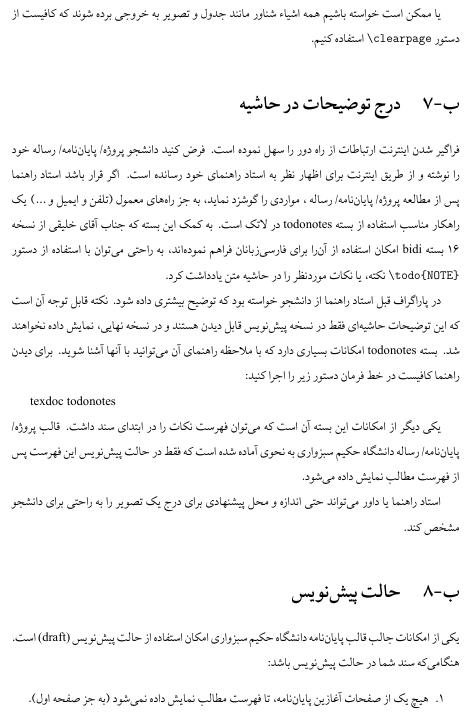
\includegraphics[width=.445\textwidth]{nodraft}}
\subfigure[حالت پیش‌نویس]{ \label{fig:draft:yes}
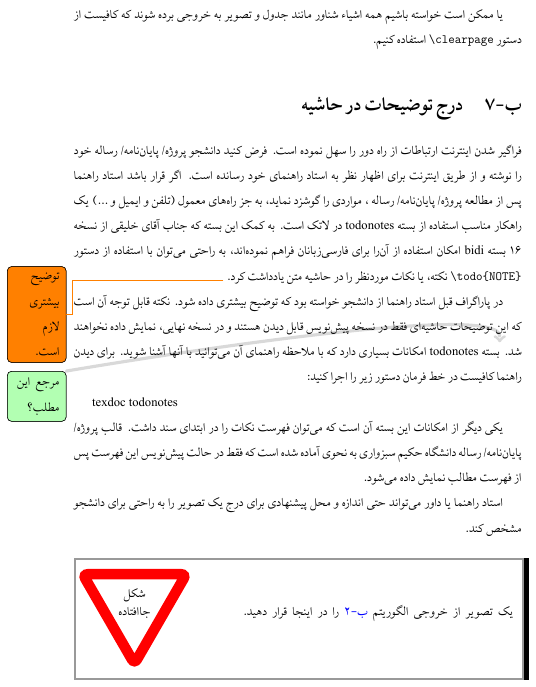
\includegraphics[width=.53\textwidth]{draft}}
\caption[مقایسه حالت معمولی و حالت پیش‌نویس]
{مقایسه خروجی بخشی از نوشتار در حالت پیش‌فرض (بدون استفاده از گزینه 
\lr{draft}) و حالت پیش‌نویس
\lr{(draft)}}
\label{fig:draft} %% label for entire figure
\end{figure}

%\newpage
%\setLTRparagraphfootnotes
%در اینجا یک زیرنویس چپ به راست را امتحان می‌کنم
%\LTRfootnote{Footnote}.

		

% !TEX TS-program = XeLaTeX
% !TeX root=main.tex
\chapter*{واژه‌نامه فارسی به انگلیسی}\markboth{واژه‌نامه فارسی به انگلیسی}{واژه‌نامه فارسی به انگلیسی}
\addcontentsline{toc}{chapter}{واژه‌نامه فارسی به انگلیسی}


\englishgloss{Probabilistic}{احتمالی}
\englishgloss{Valuation}{ارزیابی}
\englishgloss{Measure}{اندازه }
\englishgloss{Stably}{پایدار}
\englishgloss{Weak Topology}{توپولوژی ضعیف}
\englishgloss{Powerdomain}{دامنه توانی}
\englishgloss{Function Space}{فضای تابع}
\englishgloss{Semantic Domain}{دامنه معنایی}
\englishgloss{Program Fragment}{قطعه برنامه}
\englishgloss{Dcpo}{مجموعه جزئاً مرتب کامل جهت دار}
\englishgloss{Ordered}{مرتب}
% !TEX TS-program = XeLaTeX
% !TeX root=main.tex
\chapter*{واژه‌نامه  انگلیسی به  فارسی}\markboth{واژه‌نامه  انگلیسی به  فارسی}{واژه‌نامه  انگلیسی به  فارسی}
\addcontentsline{toc}{chapter}{واژه‌نامه  انگلیسی به  فارسی}


\persiangloss{مجموعه جزئاً مرتب کامل جهت دار}{Dcpo}
\persiangloss{فضای تابع}{Function Space}
\persiangloss{اندازه }{Measure}
\persiangloss{مرتب}{Ordered}
\persiangloss{دامنه توانی}{Powerdomain}
\persiangloss{احتمالی}{Probabilistic}
\persiangloss{قطعه برنامه}{Program Fragment}
\persiangloss{دامنه معنایی}{Semantic Domain}
\persiangloss{پایدار}{Stably}
\persiangloss{ارزیابی}{Valuation}
\persiangloss{توپولوژی ضعیف}{Weak Topology}


\printindex
% !TEX TS-program = XeLaTeX
% !TeX root=main.tex
% در این فایل، عنوان پایان‌نامه، مشخصات خود و چکیده پایان‌نامه را به انگلیسی، وارد کنید.

%%%%%%%%%%%%%%%%%%%%%%%%%%%%%%%%%%%%
\baselineskip=.6cm
\begin{latin}
\latinuniversity{Hakim Sabzevari University}
\latinfaculty{Faculty of Mathematics and Computer Science}
\latinsubject{Applied Mathematics}
\latinfield{Operational Research}
\latintitle{Writing projects, theses and dissertations using HSU-Thesis Class}
\firstlatinsupervisor{Dr. Mehdi Zaferanieh}
%\secondlatinsupervisor{Second Supervisor}
\firstlatinadvisor{Dr. Alireza Ghodsi}
%\secondlatinadvisor{Second Advisor}
\latinname{Mahmood}
\latinsurname{Amintoosi}
\latinthesisdate{August 2016}
\latinkeywords{Writing Thesis, Template, \LaTeX, \XePersian}
\en-abstract{
Graduate students who will be submitting a dissertation or research master’s thesis should familiarize themselves with the Graduate School’s formatting requirements and deadlines for submission.
This thesis document class is used to produce either a master's or a doctoral thesis that meets the formatting requirments of the Graduate School without any knowledge about formatting requirements.
This thesis studies on writing projects, theses and dissertations using HSU-Thesis Class. 
}
\label{LastPage}

\latinfirstPage
\end{latin}


\end{document}